%% LyX 2.4.3 created this file.  For more info, see https://www.lyx.org/.
%% Do not edit unless you really know what you are doing.
\documentclass[journal,article,submit,pdftex,moreauthors]{Definitions/mdpi}
\usepackage[utf8]{inputenc}
\usepackage{float}
\usepackage{url}
\usepackage{amstext}
\usepackage{graphicx}

\makeatletter

%%%%%%%%%%%%%%%%%%%%%%%%%%%%%% LyX specific LaTeX commands.

\Title{Predicting the forest fire duration enriched with meteorological data
using Feature Construction Techniques}

\TitleCitation{Predicting the forest fire duration enriched with meteorological data
using Feature Construction Techniques}

\Author{Constantina Kopitsa$^{1}$, Ioannis G. Tsoulos$^{2*}$, Andreas Miltiadous$^{3}$,
Vasileios Charilogis$^{4}$}

\AuthorNames{Constantina Kopitsa, Ioannis G. Tsoulos, Andreas Miltiadous and Vasileios
Charilogis}

\AuthorCitation{Kopitsa, C.; Tsoulos, I.G.;Miltiadous, A.;Charilogis V.}


\address{$^{1}$\quad{}Department of Informatics and Telecommunications,
University of Ioannina, Greece;k.kopitsa@uoi.gr\\
$^{2}$\quad{}Department of Informatics and Telecommunications, University
of Ioannina, Greece; itsoulos@uoi.gr\\
$^{3}\quad$Department of Informatics and Telecommunications, University
of Ioannina, Greece; a.miltiadous@uoi.gr\\
$^{4}\quad$Department of Informatics and Telecommunications, University
of Ioannina, Greece; v.charilog@uoi.gr}


\corres{Correspondence: itsoulos@uoi.gr}


\abstract{The spread of contemporary artificial intelligence technologies,
particularly Machine Learning, has significantly enhanced the capacity
to predict natural disasters. Wildfires constitute a prominent example,
as machine learning can be employed to forecast not only their spatial
extent but also their environmental and socio-economic impacts, propagation
dynamics, and even their duration. Such predictive capabilities are
of critical importance for effective wildfire management, as they
inform the strategic allocation of material resources, and the optimal
deployment of human personnel in the field. The necessity of leveraging
machine learning tools has become imperative in our era, as climate
change has disrupted traditional wildfire management models due to
prolonged droughts, rising temperatures, and the increasing frequency
of extreme weather events. For this reason, our research seeks to
fully exploit the potential of Principal Component Analysis (PCA),
Minimum Redundancy Maximum Relevance (MRMR), and Grammatical Evolution,
both for constructing Artificial Features and for generating Neural
Network Architectures. For this purpose, we utilized the highly detailed
and publicly available datasets provided by the Hellenic Fire Service
for the years 2014--2021, which we further enriched with meteorological
data, corresponding to the prevailing conditions at both the onset,
and the suppression of each wildfire event. The research concluded
that the Feature Construction technique, using Grammatical Evolution,
outperforms other methods in terms of stability and accuracy. Specifically,
the model accuracy of wildfire duration using Feature Construction,
the mean error was 8.79\%, indicating an overall accuracy of 91.21\%.}


\keyword{Forest fires; Machine learning; Neural networks; Feature Construction;
Genetic Programming; Grammatical Evolution}

\DeclareTextSymbolDefault{\textquotedbl}{T1}
%% Because html converters don't know tabularnewline
\providecommand{\tabularnewline}{\\}

%%%%%%%%%%%%%%%%%%%%%%%%%%%%%% Textclass specific LaTeX commands.
\newenvironment{lyxcode}
	{\par\begin{list}{}{
		\setlength{\rightmargin}{\leftmargin}
		\setlength{\listparindent}{0pt}% needed for AMS classes
		\raggedright
		\setlength{\itemsep}{0pt}
		\setlength{\parsep}{0pt}
		\normalfont\ttfamily}%
	 \item[]}
	{\end{list}}

%%%%%%%%%%%%%%%%%%%%%%%%%%%%%% User specified LaTeX commands.
%  LaTeX support: latex@mdpi.com 
%  For support, please attach all files needed for compiling as well as the log file, and specify your operating system, LaTeX version, and LaTeX editor.

%=================================================================


% For posting an early version of this manuscript as a preprint, you may use "preprints" as the journal and change "submit" to "accept". The document class line would be, e.g., \documentclass[preprints,article,accept,moreauthors,pdftex]{mdpi}. This is especially recommended for submission to arXiv, where line numbers should be removed before posting. For preprints.org, the editorial staff will make this change immediately prior to posting.

%--------------------
% Class Options:
%--------------------
%----------
% journal
%----------
% Choose between the following MDPI journals:
% acoustics, actuators, addictions, admsci, adolescents, aerospace, agriculture, agriengineering, agronomy, ai, algorithms, allergies, alloys, analytica, animals, antibiotics, antibodies, antioxidants, applbiosci, appliedchem, appliedmath, applmech, applmicrobiol, applnano, applsci, aquacj, architecture, arts, asc, asi, astronomy, atmosphere, atoms, audiolres, automation, axioms, bacteria, batteries, bdcc, behavsci, beverages, biochem, bioengineering, biologics, biology, biomass, biomechanics, biomed, biomedicines, biomedinformatics, biomimetics, biomolecules, biophysica, biosensors, biotech, birds, bloods, blsf, brainsci, breath, buildings, businesses, cancers, carbon, cardiogenetics, catalysts, cells, ceramics, challenges, chemengineering, chemistry, chemosensors, chemproc, children, chips, cimb, civileng, cleantechnol, climate, clinpract, clockssleep, cmd, coasts, coatings, colloids, colorants, commodities, compounds, computation, computers, condensedmatter, conservation, constrmater, cosmetics, covid, crops, cryptography, crystals, csmf, ctn, curroncol, currophthalmol, cyber, dairy, data, dentistry, dermato, dermatopathology, designs, diabetology, diagnostics, dietetics, digital, disabilities, diseases, diversity, dna, drones, dynamics, earth, ebj, ecologies, econometrics, economies, education, ejihpe, electricity, electrochem, electronicmat, electronics, encyclopedia, endocrines, energies, eng, engproc, ent, entomology, entropy, environments, environsciproc, epidemiologia, epigenomes, est, fermentation, fibers, fintech, fire, fishes, fluids, foods, forecasting, forensicsci, forests, foundations, fractalfract, fuels, futureinternet, futureparasites, futurepharmacol, futurephys, futuretransp, galaxies, games, gases, gastroent, gastrointestdisord, gels, genealogy, genes, geographies, geohazards, geomatics, geosciences, geotechnics, geriatrics, hazardousmatters, healthcare, hearts, hemato, heritage, highthroughput, histories, horticulturae, humanities, humans, hydrobiology, hydrogen, hydrology, hygiene, idr, ijerph, ijfs, ijgi, ijms, ijns, ijtm, ijtpp, immuno, informatics, information, infrastructures, inorganics, insects, instruments, inventions, iot, j, jal, jcdd, jcm, jcp, jcs, jdb, jeta, jfb, jfmk, jimaging, jintelligence, jlpea, jmmp, jmp, jmse, jne, jnt, jof, joitmc, jor, journalmedia, jox, jpm, jrfm, jsan, jtaer, jzbg, kidney, kidneydial, knowledge, land, languages, laws, life, liquids, literature, livers, logics, logistics, lubricants, lymphatics, machines, macromol, magnetism, magnetochemistry, make, marinedrugs, materials, materproc, mathematics, mca, measurements, medicina, medicines, medsci, membranes, merits, metabolites, metals, meteorology, methane, metrology, micro, microarrays, microbiolres, micromachines, microorganisms, microplastics, minerals, mining, modelling, molbank, molecules, mps, msf, mti, muscles, nanoenergyadv, nanomanufacturing, nanomaterials, ncrna, network, neuroglia, neurolint, neurosci, nitrogen, notspecified, nri, nursrep, nutraceuticals, nutrients, obesities, oceans, ohbm, onco, oncopathology, optics, oral, organics, organoids, osteology, oxygen, parasites, parasitologia, particles, pathogens, pathophysiology, pediatrrep, pharmaceuticals, pharmaceutics, pharmacoepidemiology, pharmacy, philosophies, photochem, photonics, phycology, physchem, physics, physiologia, plants, plasma, pollutants, polymers, polysaccharides, poultry, powders, preprints, proceedings, processes, prosthesis, proteomes, psf, psych, psychiatryint, psychoactives, publications, quantumrep, quaternary, qubs, radiation, reactions, recycling, regeneration, religions, remotesensing, reports, reprodmed, resources, rheumato, risks, robotics, ruminants, safety, sci, scipharm, seeds, sensors, separations, sexes, signals, sinusitis, skins, smartcities, sna, societies, socsci, software, soilsystems, solar, solids, sports, standards, stats, stresses, surfaces, surgeries, suschem, sustainability, symmetry, synbio, systems, taxonomy, technologies, telecom, test, textiles, thalassrep, thermo, tomography, tourismhosp, toxics, toxins, transplantology, transportation, traumacare, traumas, tropicalmed, universe, urbansci, uro, vaccines, vehicles, venereology, vetsci, vibration, viruses, vision, waste, water, wem, wevj, wind, women, world, youth, zoonoticdis 

%---------
% article
%---------
% The default type of manuscript is "article", but can be replaced by: 
% abstract, addendum, article, book, bookreview, briefreport, casereport, comment, commentary, communication, conferenceproceedings, correction, conferencereport, entry, expressionofconcern, extendedabstract, datadescriptor, editorial, essay, erratum, hypothesis, interestingimage, obituary, opinion, projectreport, reply, retraction, review, perspective, protocol, shortnote, studyprotocol, systematicreview, supfile, technicalnote, viewpoint, guidelines, registeredreport, tutorial
% supfile = supplementary materials

%----------
% submit
%----------
% The class option "submit" will be changed to "accept" by the Editorial Office when the paper is accepted. This will only make changes to the frontpage (e.g., the logo of the journal will get visible), the headings, and the copyright information. Also, line numbering will be removed. Journal info and pagination for accepted papers will also be assigned by the Editorial Office.

%------------------
% moreauthors
%------------------
% If there is only one author the class option oneauthor should be used. Otherwise use the class option moreauthors.

%---------
% pdftex
%---------
% The option pdftex is for use with pdfLaTeX. If eps figures are used, remove the option pdftex and use LaTeX and dvi2pdf.

%=================================================================
% MDPI internal commands - do not modify
\firstpage{1} 
 
\setcounter{page}{\@firstpage} 

\pubvolume{1}
\issuenum{1}
\articlenumber{0}
\pubyear{2024}
\copyrightyear{2024}
%\externaleditor{Academic Editor: Firstname Lastname} % For journal Automation, please change Academic Editor to "Communicated by"
\datereceived{}
\daterevised{ } % Comment out if no revised date
\dateaccepted{}
\datepublished{}
%\datecorrected{} % Corrected papers include a "Corrected: XXX" date in the original paper.
%\dateretracted{} % Corrected papers include a "Retracted: XXX" date in the original paper.
\hreflink{https://doi.org/} % If needed use \linebreak
%\doinum{}
%------------------------------------------------------------------
% The following line should be uncommented if the LaTeX file is uploaded to arXiv.org
%\pdfoutput=1

%=================================================================
% Add packages and commands here. The following packages are loaded in our class file: fontenc, inputenc, calc, indentfirst, fancyhdr, graphicx, epstopdf, lastpage, ifthen, lineno, float, amsmath, setspace, enumitem, mathpazo, booktabs, titlesec, etoolbox, tabto, xcolor, soul, multirow, microtype, tikz, totcount, changepage, attrib, upgreek, cleveref, amsthm, hyphenat, natbib, hyperref, footmisc, url, geometry, newfloat, caption

%=================================================================
%% Please use the following mathematics environments: Theorem, Lemma, Corollary, Proposition, Characterization, Property, Problem, Example, ExamplesandDefinitions, Hypothesis, Remark, Definition, Notation, Assumption
%% For proofs, please use the proof environment (the amsthm package is loaded by the MDPI class).

%=================================================================
% The fields PACS, MSC, and JEL may be left empty or commented out if not applicable
%\PACS{J0101}
%\MSC{}
%\JEL{}

%%%%%%%%%%%%%%%%%%%%%%%%%%%%%%%%%%%%%%%%%%
% Only for the journal Diversity
%\LSID{\url{http://}}

%%%%%%%%%%%%%%%%%%%%%%%%%%%%%%%%%%%%%%%%%%
% Only for the journal Applied Sciences:
%\featuredapplication{Authors are encouraged to provide a concise description of the specific application or a potential application of the work. This section is not mandatory.}
%%%%%%%%%%%%%%%%%%%%%%%%%%%%%%%%%%%%%%%%%%

%%%%%%%%%%%%%%%%%%%%%%%%%%%%%%%%%%%%%%%%%%
% Only for the journal Data:
%\dataset{DOI number or link to the deposited data set in cases where the data set is published or set to be published separately. If the data set is submitted and will be published as a supplement to this paper in the journal Data, this field will be filled by the editors of the journal. In this case, please make sure to submit the data set as a supplement when entering your manuscript into our manuscript editorial system.}

%\datasetlicense{license under which the data set is made available (CC0, CC-BY, CC-BY-SA, CC-BY-NC, etc.)}

%%%%%%%%%%%%%%%%%%%%%%%%%%%%%%%%%%%%%%%%%%
% Only for the journal Toxins
%\keycontribution{The breakthroughs or highlights of the manuscript. Authors can write one or two sentences to describe the most important part of the paper.}

%%%%%%%%%%%%%%%%%%%%%%%%%%%%%%%%%%%%%%%%%%
% Only for the journal Encyclopedia
%\encyclopediadef{Instead of the abstract}
%\entrylink{The Link to this entry published on the encyclopedia platform.}
%%%%%%%%%%%%%%%%%%%%%%%%%%%%%%%%%%%%%%%%%%

%%%%%%%%%%%%%%%%%%%%%%%%%%%%%%%%%%%%%%%%%%
% Only for the journal Advances in Respiratory Medicine
%\addhighlights{yes}
%\renewcommand{\addhighlights}{%

%\noindent This is an obligatory section in “Advances in Respiratory Medicine”, whose goal is to increase the discoverability and readability of the article via search engines and other scholars. Highlights should not be a copy of the abstract, but a simple text allowing the reader to quickly and simplified find out what the article is about and what can be cited from it. Each of these parts should be devoted up to 2~bullet points.\vspace{3pt}\\
%\textbf{What are the main findings?}
% \begin{itemize}[labelsep=2.5mm,topsep=-3pt]
% \item First bullet.
% \item Second bullet.
% \end{itemize}\vspace{3pt}
%\textbf{What is the implication of the main finding?}
% \begin{itemize}[labelsep=2.5mm,topsep=-3pt]
% \item First bullet.
% \item Second bullet.
% \end{itemize}
%}
%%%%%%%%%%%%%%%%%%%%%%%%%%%%%%%%%%%%%%%%%%

\makeatother

\begin{document}
\maketitle

\section{Introduction}

In this section, we begin with a brief reference to the dual role
that fire has played in shaping human civilization. Historically,
fire has possessed the capacity to either elevate civilizations or
bring about their destruction. Fire has served as a weapon capable
of unleashing unspeakable natural disasters, while simultaneously
acting as a catalyst for technological advancement. For instance,
the Great fire of London in 1666, devastated the city and reshaped
the political, social, demographic, and economical landscape\citep{Field }.
On the other hand, the ability to harness fire for cooking, metallurgy,
and warmth played a crucial role in the development, of early industrial
processes and human societies \citep{fire1}. This duality, underscores
fire’s paradoxical role, in human progress: a force capable of both
creation and destruction.

This belief is also evident in ancient Greek mythology, particularly
in the tale of Prometheus, who defied the gods by stealing fire, and
gifting it to humanity. This act symbolizes the transfer of divine
knowledge and power to humans, enabling progress and civilization.
The myth, underscores fire's dual role as a tool for human advancement
and as a source of conflict illustrating the tension between progress
and its ethical implications as well as the costs of rebellion and
innovation \citep{fire2}. In other words, fire has exerted a multiple
role in human history, both through myths and its diverse impacts. 

Thus, in the modern era, wildfires are ranked highly among the most
significant natural hazards \citep{fire3} with immense effects on
Earth's ecosystems, and human societies. Beyond that according the
Chair of ISO/TC 92 fire safety Mr. P. Van Hees: ‘\emph{With losses
caused by fire estimated at 1\% of the global GDP each year, fire
safety must be viewed in the broader perspective of risk management
and disaster mitigation}’ \citep{fire4}. 

In Figure \ref{fig:fireEconomic} it is illustrated, through a graphical
representation the economic burden from forest fires on the annual
GDP. 

\begin{figure}[H]
\begin{centering}
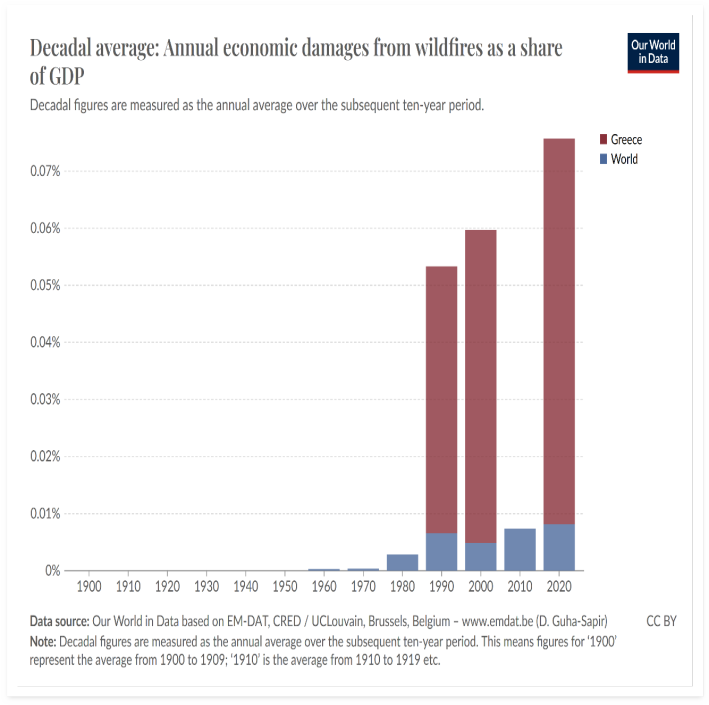
\includegraphics[scale=0.5]{fire_economic}
\par\end{centering}
\caption{The economic impact of forest fires in Greece, and around the world.\label{fig:fireEconomic}}

\end{figure}
The following numbers show the extent of the destruction caused by
fires:
\begin{itemize}
\item The cost of fire is estimated at about 1\% to 2\% of the annual GDP 
\item About 1\% of fires are responsible for more than 50\% of the costs 
\item The number of people dying in fire is estimated at 2.2 deaths per
100,000 inhabitants (based on 35 countries)\citep{fire4}. 
\end{itemize}
In other words wildfires and climate change fuel each other's intensify.
Climate change interact synergistically with wildfires by increasing
drought, high temperatures, low humidity, lightning, and strong winds,
leading to more severe, and prolonged fire seasons. Conversely, wildfires
contribute to reinforcing climate change \citep{fire5}. Thus, wildfires
(along with the extraction and burning of fossil fuels, and volcanic
eruptions) mutually enhance Climate Change, by further releasing carbon
dioxide, into the atmosphere \citep{fire_nasa}. Concerning this,
the Mediterranean region is recognized as a key \textquotedbl hot-spot\textquotedbl{}
for the forceful impacts of climate change \citep{fire_giorgi}. At
the same time, the critical need to address climate changes, effects
on wildfire patterns is highlighted as crucial for protecting both
the environment, and public health in Greece \citep{fire_iliopoulos}.

In Figure \ref{fig:fireAtmosphere}, we observe the continuous increase
in carbon dioxide levels, beginning in 1751.

\begin{figure}[H]
\begin{centering}
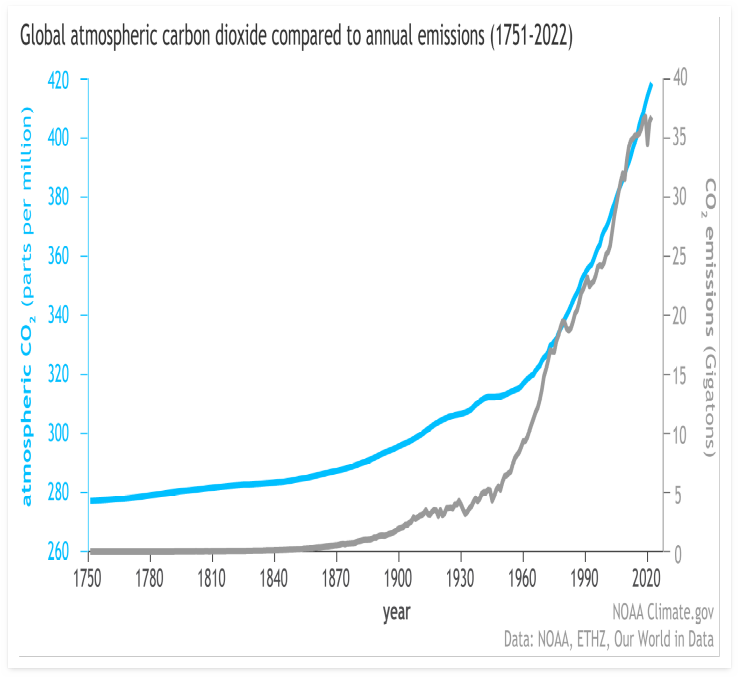
\includegraphics[scale=0.5]{fire_atmosphere}
\par\end{centering}
\caption{The environmental impact of carbon dioxide. Available from: https://www.climate.gov/news-features/understanding-climate/climate-change-atmospheric-carbon-dioxide
(accessed on November 29, 2024). \label{fig:fireAtmosphere}}

\end{figure}
 In this regard, the United Nations of Environment Programme, are
calling the governments: “to radically shift their investments in
wildfires to focus on prevention and preparedness” \citep{fire5}.
On that ground, despite the challenging conditions posed by Climate
Change, driven by endless human expansion and technological progress,
we attempt to transform this disadvantage into an advantage by focusing
our efforts on rising technology itself. That is to say, Artificial
intelligence, particularly Machine learning, emerges as a helpful
ally in addressing this global issue, offering innovative resolutions
and aiding sustainable development \citep{ai_climate,ai_ml}. 

Machine learning, apply to a collection of techniques and algorithms
that make it easier for systems to identify patterns and make decisions
based on data enriching their performance over time without explicitly
being programmed for specific tasks \citep{iso_ml}. This was the
vision, of Alan Turing, when, in 1936 he wrote his PhD ‘On Computable
Numbers, with an application to the Entscheidung problem’ \citep{ml_turing}.
That is to say, Machine learning, is a vital branch of artificial
intelligence, presents golden opportunities for businesses and society
alike. Beyond, its countless advantages it plays a critical role in
driving innovative advancements in Climate Change adaptation and mitigation.
By accelerating, the development of resolutions, to some of the most
urgent challenges facing the planet, machine learning is transforming
the process we address global environmental issues \citep{iso_ml}.
Even though, modeling multiplex environmental variables, repeatedly
presents challenges on account of significant computation resources
required and the diverseness or complexity of data formats \citep{ml_review}.
Machine learning algorithms, nevertheless, can bypass these challenges
by deriving mappings and relationships straight from the data eliminating
the need for prespecified expert rules. This ability is particularly
helpful when dealing with frameworks involving a large number of parameters
with complex physical properties, such as in forest fires. Therefore,
adopting a machine learning technique to fire management can help
defeat many of the barriers associated with traditional physics-based
simulation models.

Concerning this, in the current literature, noteworthy interest has
been developed, in the role of machine learning in the domain of fire
management \citep{fire_manage}. Forest fires, though, have not been
highly studied, as research on forest fires represent only 2.9\% of
the global literature, according to a study conducted between 2017
and 2021 \citep{fire_manage2}. More specifically, floods drawing
the most attention in research (20.3\%), followed by earthquakes and
hurricanes, each accounting for 18.8\%. Studies on general disaster
types make up 15.9\%, while landslides account for 10.1\%. Remarkably,
depending on the area of focus, researchers apply corresponding algorithms
to address specified challenges.

\begin{figure}[H]
\begin{centering}
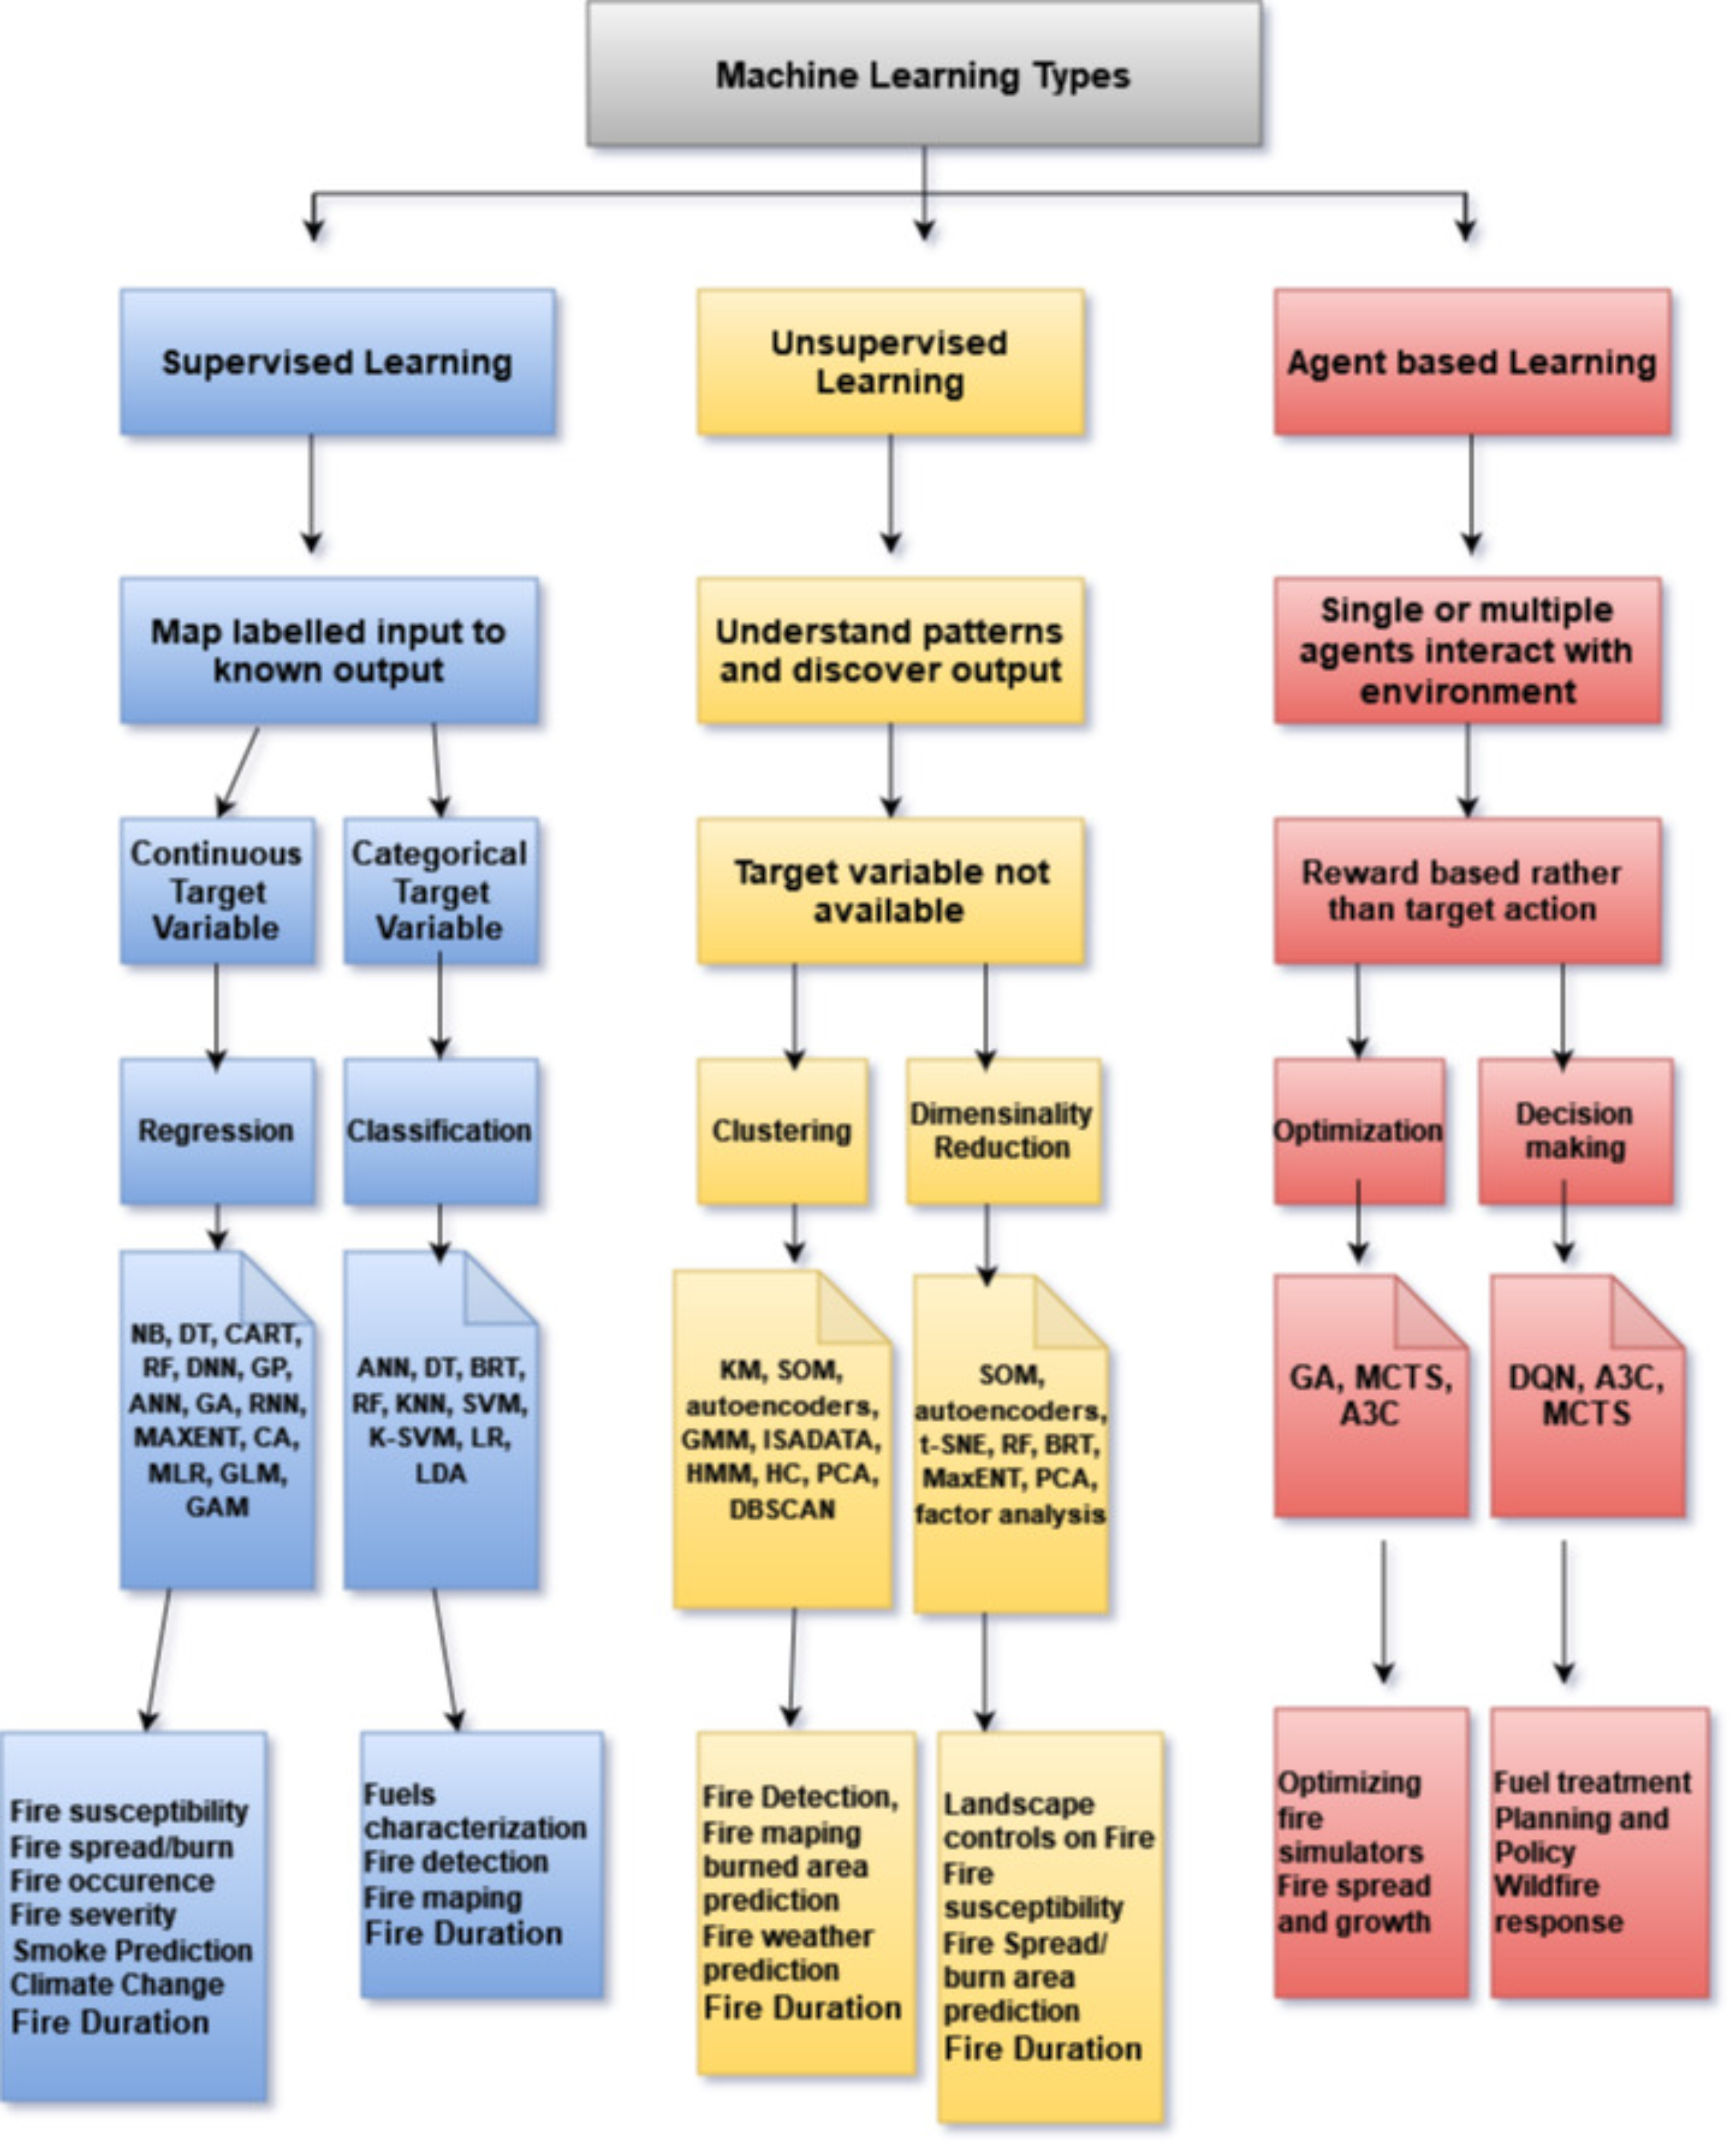
\includegraphics[scale=0.5]{fire_algorithms}
\par\end{centering}
\caption{Machine learning methods used in fire management.\label{fig:mlMethods}}

\end{figure}
Figure \ref{fig:mlMethods} sum up the machine learning methods used
in several fields of fire management, as obtained from the relevant
literature. At this point, we present a number of recent publications,
which utilize machine learning techniques for forest fire management.
For example, Bayesian networks have been broadly applied in the context
of forest fires, in particular `` A Bayesian network model for prediction
and analysis of possible forest fire causes'' \citep{fire_bayes1}.
Additionally, a recent study `` Modeling of the cascading impacts
of drought and forest fire based on a Bayesian network'' \citep{fire_bayes2}.
Also, Bayesian networks were integrated with deep learning techniques
``A Bayesian network-based information fusion combined with DNNs
for robust video fire detection'' \citep{fire_bayes3}.

Naïve Bayes, has also been employed to forest fire-related challenges
in many studies. For instance, Nugroho developed a forest fire prevention
system, ``Peatland Forest Fire Prevention Using Wireless Sensor Network
Based on Naïve Bayes Classifier'' \citep{fire_naive1}. Zainul's
work proposes a method for classifying hotspots responsible for forest
fires ``Classification of Hotspots Causing Forest and Land Fires
Using the Naive Bayes Algorithm'' \citep{fire_naive2}. Karo, present
a method for wildfire classification, that incorporates feature selection
and employs Naïve Bayes alongside other machine learning techniques
``Wildfires Classification Using Feature Selection with K-NN, Naïve
Bayes, and ID3 Algorithms'' \citep{fire_naive3}.

Moreover, Logistic Regression, has been deployed to various forest
fire-related issues, including estimating human-caused wildfire risk
``Logistic regression models for human-caused wildfire risk estimation:
analyzing the effect of the spatial accuracy in fire occurrence data''
\citep{fire_log1}, predicting wildfire vulnerability ``Predicting
wildfire vulnerability using logistic regression and artificial neural
networks: a case study in Brazil’s Federal District'' \citep{fire_log2},
probabilistic modeling of wildfire occurrence ``Probabilistic modeling
of wildfire occurrence based on logistic regression, Niassa Reserve,
Mozambique'' \citep{fire_log3} and analyzing wildfire danger ``
Analysis of Wildfire Danger Level Using Logistic Regression Model
in Sichuan Province, China''\citep{fire_log4}. 

Numerous studies, have utilized Artificial Neural Networks (ANNs),
in the area of forest fire prediction, and monitoring. For instance,
Hossain, employed ANNs to detect flames and smoke ``Wildfire flame
and smoke detection using static image features and artificial neural
network'' \citep{fire_ann1}. Lall and Mathibela applied neural networks
to predict wildfire risk ``The application of artificial neural networks
for wildfire risk prediction'' in Cape Town \citep{fire_ann2}. Likewise,
Sayad utilized neural networks along with other machine learning techniques
for wildfire predictive modeling, using data from NASA’s Land Processes
Distributed Active Archive Center (LP DAAC) ``Predictive modeling
of wildfires: A new dataset and machine learning approach'' \citep{fire_ann3}.
Similarly, Gao recently published a case study, on predicting wildfires,
in a Chinese province, `` Using multilayer perceptron to predict
forest fires in Jiangxi province, southeast china'' using neural
networks \citep{fire_ann4}. 

In addition, Random Forest, has been widely employed in forest fire
prediction. For instance, Latifah applied Random Forest, to predict
forest fires in ``Evaluation of Random Forest model for forest fire
prediction based on climatology over Borneo'' \citep{fire_rf1}.
In parallel, Malik proposed the usage of Random Forest to estimate
`` Data-driven wildfire risk prediction in northern California''
\citep{fire_rf2}. Song, demonstrated the superiority of Random Forest
model, over SVM, XGBoost, and LightGBM, in predicting forest lightning
fires ``Interpretable artificial intelligence models for predicting
lightning prone to inducing forest fires'' \citep{Song}. As well,
Gao conducted a forest fire risk prediction study in China, ``Forest-fire-risk
prediction based on random forest and back propagation neural network
of Heihe area in Heilongjiang province, China'' \citep{fire_rf3}.
Hu, developed and validated results, related to fires events in fuel
tank, employing Particle Swarm Optimization with a back propagation
neural network ``Development and Validation of a Novel Method to
Predict Flame Behavior in Tank Fires Based on CFD Modeling and Machine
Learning'' \citep{Hu}. 

This paper examines a key issue in forest fire management, such as
predicting the duration of fires, using data from already caused forest
fires in combination with the weather conditions that prevailed during
the development of this phenomenon. Concerning this topic a series
of research papers have been published during the past years, like
the work of Xiao et al \citep{fire_manage}, who designed a wildfire
duration prediction model, based on historical fire data and geospatial
information. The algorithms employed included: RF (Random Forest),
KNN, and XGBoost regression models s well as image-based approaches
such as CNN and Encoder. The model, achieved an accuracy exceeding
80\% for fires lasting longer than 10 days. In the same vein, Andela
validated the fire data from the Global Fire Atlas, utilizing independent
datasets from the United States. The study employed satellite data
and highlighted that the duration of fires is significantly influenced
among others by the fire season `` The Global Fire Atlas of individual
fire size, duration, speed and direction'' \citep{duration_andela}.
Ujjwal settled a surrogate model to capture the dynamic spread of
a wildfire over time. The mathematical model, designed to simulate
the relationship between the burned area and key meteorological parameters
(such as relative humidity, temperature, and wind speed), provides
valuable insights, into fire behavior `` A surrogate model for rapidly
assessing the size of a wildfire over time'' \citep{duration_surrogate}.
Zi-Cong, also leveraged the capabilities of a Deep Learning Surrogate
Model, designed to predict the temperature evolution, within a tunnel
in the event of a fire outbreak ``A deep learning-{}-based surrogate
model for spatial-temporal temperature field prediction in subway
tunnel fires via CFD simulation'' {[}38{]}. Liang, investigated the
capable of yielding results for predicting, wildfire duration, primarily,
focused on forecasting the scale of a forest fire. The research, ``A
neural network model for wildfire scale prediction using meteorological
factors'' utilized neural network algorithms, including Back propagation
Neural Network (BPNN), Recurrent Neural Network (RNN) and Long Short-Term
Memory (LSTM). Among them, LSTM demonstrated the highest accuracy,
achieving 90.9\% \citep{duration_wang}. Subsequent, researchers also
highlighted the LSTM method, in a study concerning fires in enclosed
and industrial environments `` Prediction method and application
of temperature distribution in typical confined space spill fires
based on deep learning'' \citep{Zhai}. Xi, established a framework,
for jointly, modeling fire duration, and size using a bivariate finite
mixture model ``Modeling the duration and size of wildfires using
joint mixture models''. Four subpopulations (normal or extreme in
duration and size) were analyzed, incorporating, variables such as:
location, month, and environmental factors. The research, revealed
a strong connection between: duration, and size, and identified key
predictors, influencing these subpopulations \citep{duration_xi}.

Predicting, the duration of a fire is crucial, as it allows for estimating
the potential risk, to the affected area and determining the necessary
human resources, for its suppression. Additionally, forest fires and
climate change are commonly ``inflamed'' highlighting their interconnection.
The Western fire chief’s association, from the U.S. emphasizes that
climate change is drastically impacting the fire season. Therefore,
fire seasons now last six to eight months, compared to the four months,
they previously spanned . Face the Facts USA reports that in the U.S.
the average duration of wildfires increased from 8 days, before 1986,
to 37 days by 2013 \citep{duration_wfca}.

The current work employs a series of Feature Construction, and selection
methods in order to improve the ability of various machine learning
techniques to predict the duration of forest fires. These methods
involve creating new, meaningful variables by combining or transforming
existing data attributes \citep{genfc1}. For example, integrating
material resources deployed during a forest fire event into a single
metric constitutes Feature Construction, enabling models, to better
capture the complexity, of fire incidents, and resource allocation.
Another example, for Feature Construction, during a forest fire, is
combining weather attributes, in order to form, a fire risk index.
Such, approaches enhance data representation, facilitating more robust,
and interpretable predictive models, in disaster management. The Feature
Construction or selection methods were applied on data collected for
the Greek case that contained weather information.

The remaining of this manuscript is divided as follows: section \ref{sec:Materials-and-Methods}
described the used dataset and it provided a detail discussion on
the used methods, section \ref{sec:Results} outlines the conducted
experiments and some statistical tests on them and finally section
\ref{sec:Conclusions} discusses some conclusions on the experimental
results.

\section{Materials and Methods\label{sec:Materials-and-Methods}}

This section initiates with a description of the used datasets and
continues with a detailed description of the used feature construction
and selection techniques, that will be applied on the datasets incorporated
in the conducted experiments.

\subsection{The used dataset }

In this research, open data provided by the Hellenic Fire Service
were utilized, available at the link \url{https://www.fireservice.gr/en_US/synola-dedomenon}.
The datasets used included information on all fires that occurred
in Greece during the years 2014--2021. The data encompassed the location
of the fire, the date and time of ignition and extinguishment, the
burned areas categorized by land type, and the firefighting forces
deployed for suppression efforts. 

The datasets comply with the European transparency legislation (Directive
2013/37/EU), ensuring that the data are unbiased in terms of type
and location, and represent all fires in the Hellenic region. The
information provided by the Hellenic Fire Service is easily accessible,
regularly updated, accurate, and comprehensive, facilitating analysis
and covering all involved entities. 

Regarding burned areas, the dataset included measurements for the
following categories: forests, forested areas, groves, grasslands,
reed beds and wetlands, agricultural lands, crop residues, and landfills. 

As for the firefighting units deployed, the dataset included measurements
for the following resources: firefighters, ground-based teams, volunteers,
military forces, other supporting units, fire trucks, service vehicles,
tankers, machinery, CL-215 aircraft, PZL aircraft, GRU aircraft, as
well as contracted helicopters and aircraft.

\subsubsection{Data Preprocessing and Weather Feature Extraction}

The first step in data preprocessing involved removing rows with missing
values. Subsequently, using the OpenCage Geocoding API, the location
data, initially formatted as \textquotedbl Municipality, Area, Address,\textquotedbl{}
were converted into geolocation data in the form of latitude and longitude
coordinates.

Next, weather information was extracted for each fire event using
the OpenWeather API, capturing data for both the ignition and extinguishment
times. OpenWeather is a widely used service that provides detailed
weather data, including historical, real-time, and forecasted weather
information. The extracted weather features included the following:
\begin{enumerate}
\item \textbf{Temperature at 2 meters}: The air temperature near the ground
level.
\item \textbf{Relative Humidity at 2 meters}: The percentage of moisture
in the air relative to its maximum capacity.
\item \textbf{Dew Point at 2 meters}: The temperature at which air reaches
saturation and moisture condenses.
\item \textbf{Precipitation}: The amount of rainfall during the specific
time interval.
\item \textbf{Weather Code}: A classification of the general weather conditions
(e.g., clear, cloudy, rainy).
\item \textbf{Cloud Cover}: The percentage of the sky obscured by clouds.
\item \textbf{Evapotranspiration} (ET0): The potential evapotranspiration
measured using the FAO Penman-Monteith method, indicating water loss
from the surface and vegetation.
\item \textbf{Vapour Pressure Deficit} (VPD): The difference between the
amount of moisture in the air and the maximum it can hold.
\item \textbf{Wind Speed} at 10m and 100m: Wind velocity measured at heights
of 10 meters and 100 meters.
\item \textbf{Wind Direction} at 10m and 100m: The directional angle of
the wind at the respective heights.
\end{enumerate}
\begin{quote}
Additionally, daily-level weather data were included, such as:
\end{quote}
\begin{enumerate}
\item \textbf{Daylight Duratio}n: The total hours of daylight during the
day.
\item \textbf{Sunshine Duration}: The total hours of direct sunlight during
the day.
\end{enumerate}
\begin{quote}
These features were aggregated and matched with each fire record,
ensuring comprehensive weather context for both the ignition and extinguishment
phases of the fires.
\end{quote}

\subsubsection{Definition of the output variable}

To define the output variable, the duration of each forest fire was
converted from hours or other time units into minutes, ensuring greater
precision in classification. A logarithmic transformation of fire
duration in minutes was then applied to manage the wide range of values
effectively, preventing excessive influence from extreme durations.
Based on this transformation, three distinct categories were established,
serving as target values for experimental analysis. This approach
enabled the classification of forest fires according to their duration.
For the Greek forest fire data used in this study, the following classification
scheme was adopted: 
\begin{enumerate}
\item Up to 360 minutes (6 hours) is considered to be a fire, of short duration. 
\item From 361 -- 7200 minutes (6 hours -- 5 days) is a fire of medium
duration. 
\item More than 7201 minutes (5 days - and more), which is considered a
long duration fire.
\end{enumerate}

\subsection{The used feature construction and selection methods}

\subsubsection{The PCA method }

The Principal Component Analysis (PCA) technique, introduced by mathematician
Karl Pearson in 1901 \citep{pca1}, and developed by Harold Hotelling
(1933). This technique operates on the principle that when data from
a higher-dimensional space is transformed into a lower-dimensional
space, the resulting lower-dimensional representation should retain
the maximum variance of the original data. 

Notably, it is worth mentioning that the use of PCA, on larger datasets,
became practical only after the advent of electronic computers, which
made it computationally feasible, to handle datasets, beyond trivial
sizes \citep{pca_cadima}. Continuing, with the applications of PCA,
it is a widely utilized technique in exploratory data analysis, and
machine learning, particularly, in building predictive models. It
is an unsupervised learning method, designed to analyze, the relationships
among a set of variables. Often referred to as a form of general factor
analysis, it involves regression to determine a line of best fit.
The primary objective, of PCA, is to reduce the dimensionality of
a dataset, while retaining the most significant patterns, and relationships,
among the variables, all without requiring prior knowledge, of the
target variables \citep{pca_i2}. 

Next, we will briefly reference studies, that have utilized PCA, covering
different areas, such as: statistical physics, genetic improvement,
face recognition, economic \& environmental sciences, medical prediction,
e.t.c. Explicitly, the research conducted, by Park \citep{pca_park},
highlights the reasons behind the success of the PCA technique, for
lattice systems. The study's primary limitation lies in the dependency
of the proposed formula's accuracy on the dataset size. Specifically,
the results achieve full precision, only under the condition of an
infinite dataset. This constraint restricts the practical applicability,
of the method, when working with finite or limited data, a common
scenario, in real-world analyses. 

Additionally, the work of Sarma et al. \citep{pca_sarma} utilizes
PCA, in order to evaluate, morphometric traits, under a multivariate
approach. The findings suggest, that PCA could significantly enhance
the genetic improvement. Noteworthy, is the fact, that the 64.29\%,
of the total variance explained, can be considered relatively low.
This suggests, that a significant amount of unexplained information
remains, which is not captured, by the four principal components.
Moreover, Gambardella et al. used the PCA technique for monitoring
the cultivation, of cannabis, in Albania. Specifically, with PCA they
remove redundant spectral information from multiband datasets \citep{pca_parente}.
The article, by Slavkovic and Jevtic \citep{pca_electric}, presents
the implementation of a face recognition system based on the Principal
Component Analysis (PCA) algorithm. The PCA technique was utilized
by Hargreaves \citep{pca_stock}, for stock selection, specifically
to identify, a limited number of stock variables, that could effectively
aid, in determining winning stocks. 

Moreover, Xu et al. presents an interesting example of a modified
application of Principal Component Analysis (PCA), utilizing, both
linear and non-linear methods, through Kernel PCA (KPCA), in combination,
with the Adaptive Boosting (AdaBoost) algorithm \citep{pca_kernel}.
In the study of Zhang \citep{pca_zhang}, a neural network model,
combining PCA and Levenberg-Marquardt \citep{lm_paper} was developed,
to efficiently, and accurately analyze, and predict the interaction
between IAQ and its influencing factors. In particular, it was examined
indoor air quality (IAQ), and its relationship, with building features,
and environmental conditions. 

In the work of Akinnuwesi et al \citep{pca_svm}, a hybrid approach
was suggested combining Principal Component Analysis (PCA), and Support
Vector Machine (SVM) \citep{svm}. They create, the Breast Cancer
Risk Assessment and Early Diagnosis (BC-RAED) model, designed to accurately
detect BCa, in its early stages. PCA, was initially applied to extract
features, during the first preprocessing stage, followed by further
feature reduction, in the second stage. The multi-preprocessed data,
were analyzed for breast cancer risk, and diagnosis using SVM. The
BC-RAED model, achieved, an accuracy of 97.62\%, a sensitivity of
95.24\%, and a specificity of 100\% in assessing, and diagnosing breast
cancer risk. 

Subsequently, we will briefly mention certain studies, that have been
conducted, in the field of Forest Fires. Guan's research focuses on
forest fire prediction using PCA-preprocessed data. The preprocessing
step removed irrelevant information, simplifying analysis. Linear
regression and random forest methods were then applied, revealing
temperature, relative humidity, wind, and rain as the most influential
factors in forest fire occurrence \citep{pca_guan}. 

A novel model was developed, by Nikolov, using meteorological forecast
data as input. Principal Component Analysis (PCA), with orthogonal
rotation, was applied to reduce 195 meteorological variables, from
the NARR dataset, to a smaller set of significant fire-ignition predictors,
later used in logistic regression, to calculate wildfire ignition
probabilities \citep{pca_nikolov}. Also, a recent publication focuses
on predicting wildfire ignitions, caused by lightning strikes, which
account for the largest area burned annually, in the extratropical
Northern Hemisphere. Principal Component Analysis (PCA), played a
key role, in reducing 611 potential predictors, to 13 principal components,
which were used in logistic regression to identify the primary factors
influencing lightning occurrence \citep{pca_nikolov2}. 

\subsubsection{The MRMR method }

The min-redundancy max-relevance (MRMR) algorithm, introduced by Chris
Ding and Hanchuan Peng \citep{mrmr1}. This method aims to optimize
feature selection, by minimizing redundancy, and maximizing relevance
\citep{mrmr2}. In sum, MRMR enhances relevance-only methods, such
as using an f-test between the target, and the features. When two
features are similar, MRMR prioritizes only the one, with the highest
relevance.

The study, by Zhao, extends traditional MRMR methods, by introducing
a non-linear feature redundancy measure and a model-based feature
relevance measure, which are tested on synthetic and real-world datasets.
Based on its empirical success, MRMR is integrated into Uber's marketing
machine learning platform to automate the creation and deployment
of scalable targeting and personalization models \citep{mrmr_zhao}. 

Moreover, Wu et al. proposed that the MRMR algorithm is utilized in
conjunction with a Random Forest model \citep{random_forest} to perform
feature selection in the context of air quality prediction. MRMR,
is employed to determine which variables have the most significant
impact, on the air quality index (AQI), while minimizing redundancy
among them \citep{mrmr_wu}. 

The article, by Elbeltagi is an innovative approach for estimating
maize chlorophyll by integrating hyperspectral indices with cutting-edge,
six advanced machine learning techniques. The MRMR algorithm was incorporated
into the process to enhance feature selection by pinpointing the most
significant spectral bands, minimizing data redundancy and boosting
model efficiency \citep{mrmr_elbeltagi}. 

In the energy sector, Liu conducted the following research offering
an improved method for predicting transient stability in power systems.
The MRMR algorithm is applied for feature selection with minimal redundancy
and maximum relevance providing an enhanced approach for forecasting
transient stability, in power systems. This approach addresses the
limitations of previous methods, such as low accuracy, difficult applicability
and high computational cost, while incorporating the \textquotedbl winner
take all\textquotedbl{} (WTA) technique for ensemble learning and
enhanced precision \citep{mrmr_liu}. 

Eristi also refers to the energy sector. Specifically, this paper
presents, a new PD detection system, that combines spectral analysis,
spectrogram analysis, deep learning algorithms, MRMR and ensemble
machine learning (EML) \citep{eml}. The most impactful features,
are identified, by performing MRMR feature selection analysis, on
the extracted deep features \citep{mrmr_eristi}.

Zhang employed an Acoustic Emission (AE) technique to monitor inaccessible
areas of large storage tank floors utilizing AE sensors positioned
externally to the tank. The implemented algorithm effectively distinguishes
corrosion signals from interference signals, particularly drop-back
signals induced by condensation. Experimental studies were conducted
both in laboratory settings and in field environments, focusing on
Q235 steel. Seven characteristic AE features derived from signal hits
and frequency were extracted and subsequently selected for pattern
recognition, using the MRMR method \citep{mrmr_zhang}. 

Additionally, Karamouz et al., proposed a methodology to examine the
effects of climate change on sea level variations in coastal areas
using an artificial neural network model. Feature selection techniques,
including MRMR and Mutual Information (MI) are employed to identify
the most suitable predictors for the neural network input \citep{mrmr_razmi}. 

\subsubsection{The Neural Network Construction method }

Another machine learning method introduced recently that is based
on Grammatical Evolution \citep{ge1} is the construction of artificial
neural networks \citep{nnc}. In this work the architecture of the
neural network is produced through a series of generations of the
underlying genetic algorithm by reducing the training error of the
neural network. Furthermore, the method is able to identify the best
set of parameters for the neural network. This method can also retain
only a small portion of features from the original objective problem,
significantly reducing the information required to reduce the training
error. This method was used in a series of practical problems, such
as the identification of amide I bonds \citep{nnc_amide1}, solution
of differential equations \citep{nnc_de},\textbf{ }incorporation
in the detection of Parkinson's disease \citep{nnc_feas},\textbf{
}usage in the estimation of performance of students \citep{nnc_student},
autism screening \citep{nnc_autism} etc. 

The used grammar for the construction of neural networks expressed
in Backus--Naur (BNF) form \citep{bnf1} is shown in Figure\textbf{
}\ref{fig:nncGrammar}. Numbers in parentheses represent the sequence
number of each production rule. The constant $n$ stands for the number
of input features.{\bfseries{}
\begin{figure}[H]
\begin{lyxcode}
\textbf{S:=\textless sigexpr\textgreater ~~~~~~~~~~~~~~~~~~~~~~~~~~(0)}

\textbf{\textless sigexpr\textgreater ::=\textless Node\textgreater ~~~~~~~~~~~~~~~~~~~~(0)}

\textbf{~~~~~~~~~~~\textbar ~\textless Node\textgreater ~+~\textless sigexpr\textgreater ~~~~~~~(1)}

\textbf{\textless Node\textgreater ::=\textless number\textgreater{*}sig(\textless sum\textgreater +\textless number\textgreater )~(0)}

\textbf{\textless sum\textgreater ::=~\textless number\textgreater{*}\textless xxlist\textgreater ~~~~~~~~~~~~(0)}

\textbf{~~~~~~~~~~~\textbar ~~~~\textless sum\textgreater +\textless sum\textgreater ~~~~~~~~~~~(1)}

\textbf{\textless xxlist\textgreater ::=~x1~~~~~~~~(0)}

\textbf{~~~~~~~~~~~~~\textbar ~~~~x2~~(1)}

\textbf{~~~~~~~~~~~~~..............}

\textbf{~~~~~~~~~~~~~\textbar ~~~~xn~~(n-1)}

\textbf{\textless number\textgreater ::=~(\textless digitlist\textgreater .\textless digitlist\textgreater )~~~~~~~~(0)}

\textbf{~~~~~~~~~~~~~\textbar ~~~~(-\textless digitlist\textgreater .\textless digitlist\textgreater )~(1)}

\textbf{\textless digitlist\textgreater ::=~\textless digit\textgreater ~~~~~~~~~~~~(0)}

\textbf{~~~~~~~~~~~~~\textbar ~\textless digit\textgreater\textless digitlist\textgreater ~(1)}

\textbf{\textless digit\textgreater ::=~0~~~~~~(0)}

\textbf{~~~~~~~~~~~~~\textbar ~~1~(1)}

\textbf{~~~~~~~~~~~~~...........}

\textbf{~~~~~~~~~~~~~\textbar ~~9~(9)}
\end{lyxcode}
\textbf{\caption{The grammar incorporated in the construction of neural networks.\label{fig:nncGrammar}}
}
\end{figure}
}\textbf{ }This grammar produces artificial neural networks in the
following form:

\textbf{
\begin{equation}
\text{NN}\left(\overrightarrow{x},\overrightarrow{w}\right)=\sum_{i=1}^{H}w_{(n+2)i-(n+1)}\sigma\left(\sum_{j=1}^{n}x_{j}w_{(n+2)i-(n+1)+j}+w_{(n+2)i}\right)\label{eq:nn}
\end{equation}
}The symbol $H$ defines the number of processing nodes (weights).\textbf{
}The sigmoid function $\sigma(x)$ is used as the activation function
of neural network and it is defined as: 
\begin{equation}
\sigma(x)=\frac{1}{1+\exp(-x)}\label{eq:sig}
\end{equation}
The main steps of the algorithm are:
\begin{enumerate}
\item \textbf{Initialization step}.
\begin{enumerate}
\item \textbf{Set} the number of used chromosomes $N_{c}$. Each chromosome
is a set of randomly selected integers. These integer values represent
rule number in the extended BNF grammar previously presented.
\item \textbf{Set} the maximum number of allowed generations $N_{g}$.
\item \textbf{Set} the selection rate $p_{s}\in[0,1]$ and the mutation
rate $p_{m}\in[0,1]$.
\item \textbf{Set} $k=0$, the generation number.
\end{enumerate}
\item \textbf{Fitness calculation step}.
\begin{enumerate}
\item \textbf{For} each chromosome $g_{i},\ $$i=1,\ldots,N_{c}$ \textbf{do}
\begin{enumerate}
\item \textbf{Create} using the grammar of figure \ref{fig:nncGrammar}
the corresponding neural network $\mbox{NN}_{i}\left(\overrightarrow{x},\overrightarrow{w}\right)$
\item \textbf{Set} as $f_{i}=\sum_{j=1}^{M}\left(\mbox{NN}_{i}\left(\overrightarrow{x}_{j},\overrightarrow{w_{i}}\right)-y_{j}\right)^{2}$
the fitness of chromosome $i$. The set $\left(\overrightarrow{x_{j}},y_{j}\right),\ j=1,...,M$
stands for the train set of the objective problem.
\end{enumerate}
\item \textbf{End For}
\end{enumerate}
\item \textbf{Genetic operations step}.
\begin{enumerate}
\item Application of Selection operator. The chromosomes of the population
are sorted according to their fitness values and the best $\left(1-p_{s}\right)\times N_{c}$
chromosomes are copied to the next generation. The remaining are replaced
by new chromosomes produced during crossover and mutation.
\item Application of Crossover operator. In this step $p_{s}\times N_{c}$
new chromosomes will be created from the original ones. For each set
$c_{1},\ c_{2}$ of new chromosomes that will be created, two chromosomes
$g_{a}$ and $g_{b}$ are selected from the old population using tournament
selection. The new chromosomes are created using one - point crossover
between $g_{a}$ and $g_{b}$. An example of this operation is shown
graphically in Figure \ref{fig:onePoint}. 
\item Application of Mutation operator. For each element of every chromosome
a random number $r\in[0,1]$ is selected. The corresponding element
is changed randomly when $r\le p_{m}$.
\end{enumerate}
\item \textbf{Termination check step}.
\begin{enumerate}
\item \textbf{Set} $k=k+1$
\item \textbf{If} $k\le N_{g}$ then goto Fitness Calculation Step.
\end{enumerate}
\item \textbf{Application to the test set}.
\begin{enumerate}
\item \textbf{Obtain} the best chromosome $g^{*}$ from the genetic population.
\item \textbf{Create} the corresponding neural network $\mbox{NN}^{*}\left(\overrightarrow{x},\overrightarrow{w}\right)$
\item \textbf{Apply} this neural network to the test set of the objective
problem and report the corresponding error (test error).
\end{enumerate}
\end{enumerate}
\begin{figure}[H]
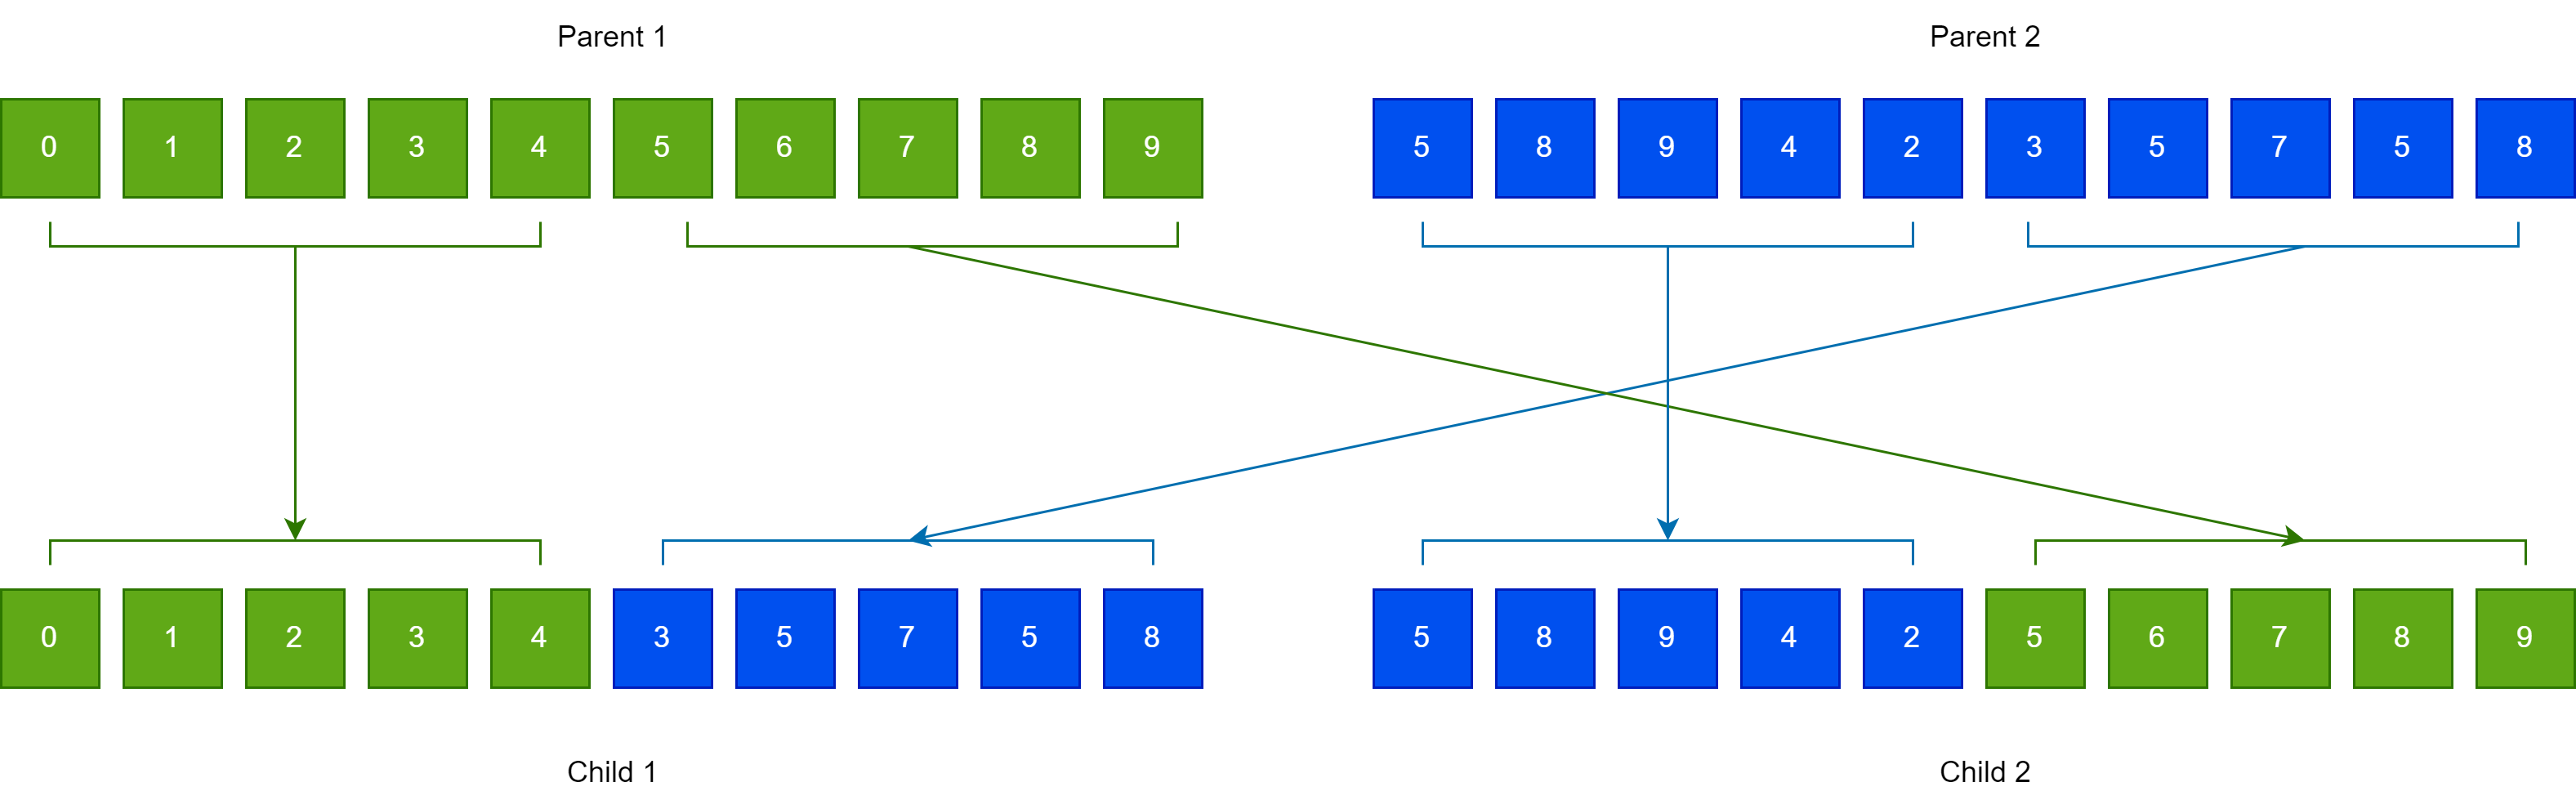
\includegraphics[scale=0.5]{onePointCrossover}

\caption{An example of the one - point crossover operation used in Grammatical
Evolution.\label{fig:onePoint}}

\end{figure}


\subsubsection{The Feature Construction method}

Another approach discussed here and used in the conducted experiments
is the feature construction technique initially proposed in \citep{fc1}.\textbf{
}This approach creates artificial features from the original ones
using the Grammatical Evolution procedure. The new features are non
- linear mappings of the original ones. This method has been used
in a series of practical cases during the past years, such as Spam
Identification \citep{fc2}, Fetal heart classification \citep{fc3},
EEG signal processing \citep{fc4,fc5} etc. The extended version of
BNF grammar used during the feature construction process is outlined
in Figure \ref{fig:fcGrammar}.

\begin{figure}[H]
\caption{The extended BNF grammar used in the feature construction process.\label{fig:fcGrammar}}

\begin{lyxcode}
S::=\textless expr\textgreater ~~~(0)~

\textless expr\textgreater ~::=~~(\textless expr\textgreater ~\textless op\textgreater ~\textless expr\textgreater )~~(0)~~~~~~~~~~~~~

~~~~~~~~~~~\textbar ~\textless func\textgreater ~(~\textless expr\textgreater ~)~~~~(1)~~~~~~~~~~~~~

~~~~~~~~~~~\textbar\textless terminal\textgreater ~~~~~~~~~~~~(2)~

\textless op\textgreater ~::=~~~~~+~~~~~~(0)~~~~~~~~~~~~~

~~~~~~~~~~~\textbar ~-~~~~~~(1)~~~~~~~~~~~~~

~~~~~~~~~~~\textbar ~{*}~~~~~~(2)~~~~~~~~~~~~~

~~~~~~~~~~~\textbar ~/~~~~~~(3)

\textless func\textgreater ~::=~~~sin~~(0)~~~~~~~~~~~~~

~~~~~~~~~~~\textbar ~cos~~(1)~~~~~~~~~~~~~

~~~~~~~~~~~\textbar exp~~~(2)~~~~~~~~~~~~~

~~~~~~~~~~~\textbar log~~~(3)

\textless terminal\textgreater ::=\textless xlist\textgreater ~~~~~~~~~~~~~~~~(0)~~~~~~~~~~~~~~~~~~~~~~

~~~~~~~~~~~\textbar\textless digitlist\textgreater .\textless digitlist\textgreater ~(1)

\textless xlist\textgreater ::=x1~~~~(0)~~~~~~~~~~~~~~

~~~~~~~~~~~\textbar ~x2~(1)~~~~~~~~~~~~~~

~~~~~~~~~~~………~~~~~~~~~~~~~

~~~~~~~~~~~\textbar ~xn~(n-1)

\textless digitlist\textgreater ::=\textless digit\textgreater ~~~~~~~~~~~~~~~~~~(0)~~~~~~~~~~~~~~~~~

~~~~~~~~~~~\textbar ~\textless digit\textgreater\textless digit\textgreater ~~~~~~~~~~~~(1)

~~~~~~~~~~~\textbar ~\textless digit\textgreater\textless digit\textgreater\textless digit\textgreater ~~~~~(2)

\textless digit\textgreater ~~::=~0~(0)~~~~~~~~~~~~~

~~~~~~~~~~~\textbar ~1~(1)~~~~~~~~~~~~~

~~~~~~~~~~~.......~~~~~~~~~~

~~~~~~~~~~~\textbar ~9~(9)
\end{lyxcode}
\end{figure}
The main steps of the used algorithm have as follows:
\begin{enumerate}
\item \textbf{Initialization step}.
\begin{enumerate}
\item \textbf{Define }the number of used chromosomes $N_{c}$. 
\item \textbf{Define} the maximum number of allowed generations $N_{g}$.
\item \textbf{Set} the selection rate $p_{s}\in[0,1]$ and the mutation
rate $p_{m}\in[0,1]$.
\item \textbf{Set} as $N_{f}$ the number of desired features that will
be created.
\item \textbf{Set} $k=0$, the generation number.
\end{enumerate}
\item \textbf{Fitness calculation step}.
\item \textbf{For $i=1,\ldots,N_{c}$ do}

\begin{enumerate}
\item \textbf{Create} with the assistance of Grammatical Evolution, a set
of $N_{f}$ artificial features from the original ones, for chromosome
$g_{i}$.
\item \textbf{Transform} the original train set using the previously produced
features. Represent the new set as $\mbox{TR}=\left(x_{g_{i},j},t_{j}\right),\ j=1,..M$
\item \textbf{Apply }a machine learning model denoted as $C$ on set TR
and train this model and denote as $C(x)$ the output of this model
for any input pattern $x$.
\item \textbf{Calculate} the fitness $f_{i}$ as:
\begin{equation}
f_{i}=\sum_{j=1}^{M}\left(C\left(x_{g_{i},j}\right)-t_{j}\right)^{2}
\end{equation}
The Radial Basis Function (RBF) networks \citep{rbf1,rbf2} were used
as the machine learning models $C(x)$ in the current work. This machine
learning model was chosen because of the significantly shorter training
time it requires compared to other machine learning models. 
\end{enumerate}
\item \textbf{End For}
\item \textbf{Genetic operations step. }Perform the same genetic operators
as in the case of construction neural networks, discussed previously.
\item \textbf{Termination check step}.
\begin{enumerate}
\item \textbf{Set} $k=k+1$
\item \textbf{If} $k\le N_{g}$ then goto Fitness Calculation Step.
\end{enumerate}
\item \textbf{Application to the test set}.
\begin{enumerate}
\item \textbf{Obtain} the chromosome $g^{*}$ with the lowest fitness value.
\item \textbf{Create} the $N_{f}$ artificial features that correspond to
this chromosome
\item \textbf{Apply} the $N_{f}$ features to the train set and produce
the mapped training set $\mbox{TR}=\left(x_{g_{i},j},t_{j}\right),\ j=1,..M$
\item \textbf{Train} a machine learning model on the produced training set.
An artificial neural network \citep{nn1,nn2} with $H=10$ processing
nodes is used in the current work. This neural network was trained
using a BFGS variant of Powell \citep{powell}. 
\item \textbf{Apply} the new features to the test set of the objective problem
and create the set $\mbox{TT=}\left(x_{g_{i},j},t_{j}\right),\ j=1,..K$
\item \textbf{Apply} the machine learning model on set TT and report the
test error.
\end{enumerate}
%
\end{enumerate}

\section{Results\label{sec:Results}}

The code used in the experiments was code in the C++ programming language
and for the optimization methods the freely available Optimus programming
tool was incorporated \citep{optimus} as as well as the WEKA programming
tool \citep{weka_main}.\textbf{ }The WEKA software has been incorporated
in a series of problems \citep{weka_education1,weka_education2,weka_medical1,weka_medical2}.
Each experiment was conducted 30 times, using different seed for the
random generator each time and the ten - fold cross validation procedure
was used to validate the experimental results. The values of parameters
for the used methods are shown in Table\textbf{ }\ref{tab:expr}.\textbf{
}The following notation is used in the tables presenting the experimental
results:
\begin{enumerate}
\item The column YEAR denotes the year of recording.
\item The column BAYES the application of the Naive Bayes \citep{naive_bayes}
method to the corresponding dataset.
\item The column ADAM represents the usage of the ADAM optimizer \citep{nn_adam}
for the training of a neural network with $H=10$ processing nodes.
\item The column BFGS denotes the incorporation of the BFGS optimizer \citep{powell}
to train a neural network with $H=10$ processing nodes.
\item The column MRMR denotes the results obtained by the application of
a neural network trained with the BFGS optimizer on two features selected
using the MRMR technique.
\item The column PCA stands for the results obtained by the application
of a neural network trained with the BFGS optimizer on two features
created using the PCA technique. The PCA variant implemented in MLPACK
software \citep{mlpack} was incorporated to create these features.
\item The column NNC denotes the usage of the method of Neural Network Construction
on the proposed datasets. The software that implements this method
was obtained from \citep{nnc_softx}.
\item The column FC represents the usage of the previously mentioned method
for constructing artificial features. For the purposes of this article
two artificial features were created. These features were produced
and evaluated using the QFc software \citep{qfc}.
\end{enumerate}
\begin{table}[H]
\caption{Experimental results using a series of machine learning methods for
the prediction of forest fire duration.\label{tab:expr}}

\centering{}{\footnotesize{}%
\begin{tabular}{|c|c|c|c|c|c|c|c|}
\hline 
{\footnotesize YEAR} & {\footnotesize BAYES} & {\footnotesize ADAM} & {\footnotesize BFGS} & {\footnotesize MRMR} & {\footnotesize PCA} & {\footnotesize NNC} & {\footnotesize FC}\tabularnewline
\hline 
\hline 
{\footnotesize 2014} & {\footnotesize 11.41\%} & {\footnotesize 13.00\%} & {\footnotesize 12.38\%} & {\footnotesize 9.68\%} & {\footnotesize 15.50\%} & {\footnotesize 9.21\%} & {\footnotesize 8.04\%}\tabularnewline
\hline 
{\footnotesize 2015} & {\footnotesize 10.49\%} & {\footnotesize 11.94\%} & {\footnotesize 11.25\%} & {\footnotesize 8.49\%} & {\footnotesize 15.03\%} & {\footnotesize 9.17\%} & {\footnotesize 7.51\%}\tabularnewline
\hline 
{\footnotesize 2016} & {\footnotesize 10.79\%} & {\footnotesize 12.95\%} & {\footnotesize 11.88\%} & {\footnotesize 9.45\%} & {\footnotesize 12.93\%} & {\footnotesize 10.12\%} & {\footnotesize 8.60\%}\tabularnewline
\hline 
{\footnotesize 2017} & {\footnotesize 53.36\%} & {\footnotesize 12.68\%} & {\footnotesize 12.65\%} & {\footnotesize 12.65\%} & {\footnotesize 12.64\%} & {\footnotesize 12.61\%} & {\footnotesize 12.66\%}\tabularnewline
\hline 
{\footnotesize 2018} & {\footnotesize 9.39\%} & {\footnotesize 10.48\%} & {\footnotesize 14.97\%} & {\footnotesize 9.21\%} & {\footnotesize 10.49\%} & {\footnotesize 9.29\%} & {\footnotesize 7.72\%}\tabularnewline
\hline 
{\footnotesize 2019} & {\footnotesize 7.79\%} & {\footnotesize 9.44\%} & {\footnotesize 9.66\%} & {\footnotesize 8.39\%} & {\footnotesize 9.72\%} & {\footnotesize 7.03\%} & {\footnotesize 6.62\%}\tabularnewline
\hline 
{\footnotesize 2020} & {\footnotesize 40.26\%} & {\footnotesize 9.56\%} & {\footnotesize 9.80\%} & {\footnotesize 9.55\%} & {\footnotesize 9.76\%} & {\footnotesize 9.50\%} & {\footnotesize 9.61\%}\tabularnewline
\hline 
{\footnotesize 2021} & {\footnotesize 11.81\%} & {\footnotesize 11.06\%} & {\footnotesize 12.90\%} & {\footnotesize 10.57\%} & {\footnotesize 11.03\%} & {\footnotesize 10.80\%} & {\footnotesize 9.55\%}\tabularnewline
\hline 
{\footnotesize\textbf{AVERAGE}} & {\footnotesize\textbf{19.41\%}} & {\footnotesize\textbf{11.39\%}} & {\footnotesize\textbf{11.94\%}} & {\footnotesize\textbf{9.75\%}} & {\footnotesize\textbf{12.14\%}} & {\footnotesize\textbf{9.72\%}} & {\footnotesize\textbf{8.79\%}}\tabularnewline
\hline 
\end{tabular}}{\footnotesize\par}
\end{table}
Table \ref{tab:expr} presents the percentage values of classification
error for various machine learning models from 2014 to 2021, as well
as the average error rate for each model. The analysis reveals significant
insights regarding the performance and stability of the methods. The
BAYES model exhibits the highest variability, with a particularly
high error rate in 2017 (53.36\%). This is a clear outlier, possibly
due to specific conditions in the data or the evaluation framework.
In other years, its error rates range between 7.79\% and 11.81\%.
The average error rate for BAYES is 19.41\%, the highest in the table,
indicating the lowest overall accuracy compared to the other models.
The ADAM model shows an average error rate of 11.39\%, with values
ranging from 9.44\% to 13.00\%. Its stability is evident, as there
are no significant deviations in specific years. ADAM's performance
is considered relatively good compared to other methods. The BFGS
model has an average error rate of 11.94\%, slightly higher than ADAM's.
Its error rates range from 9.66\% to 14.97\%. Although it demonstrates
stable performance, its higher average value suggests slightly lower
accuracy in certain cases. The MRMR model has an average error rate
of 9.75\%, ranking it among the most accurate methods. However, its
error rate reaches 12.65\% in 2017, while remaining low in other years,
making it a reliable option overall. The PCA model has an average
error rate of 12.14\%, which is among the highest in the table. It
shows relatively stable values, with a slight increase to 15.50\%
in 2014. Despite its generally good performance, its accuracy is lower
compared to other methods such as MRMR or FC. The NNC model has an
average error rate of 9.72\%, one of the lowest in the table. Its
values range from 7.03\% to 12.61\%, with small deviations, demonstrating
stability and reliability. The FC model has the lowest average error
rate in the table, at 8.79\%, making it the most accurate method overall.
Its error rates range between 6.62\% and 12.66\%, indicating stable
performance with minor fluctuations. In conclusion, FC is the most
accurate model, with the lowest average error rate, while BAYES demonstrates
the lowest accuracy due to its high average error rate and significant
variability. Methods such as MRMR and NNC are also reliable, with
low error rates and relatively stable performance. The observed deviations
in specific years might be related to changes in the data or evaluation
parameters.

In Figure \ref{fig:statExper}, the results of the Wilcoxon test for
pairwise comparisons of the classification models are presented, providing
valuable insights into the statistical significance of their performance
differences. Below is a more in-depth analysis, focusing on the interpretation
of results and a deeper understanding of the relationships between
the models. The overall result of the Wilcoxon test (p \textless{}
0.5) confirms that statistically significant differences exist among
the models' performances. This indicates that the models are not equivalent
in terms of their accuracy, with some clearly outperforming others.
The comparison between FC and NNC (p = 0.039) reveals a statistically
significant difference, though the p-value is relatively close to
the significance threshold (commonly p \textless{} 0.05). This suggests
that while FC outperforms NNC, the difference is not exceedingly pronounced.
This outcome might be influenced by specific data characteristics
or variations in the models' stability. The comparison between FC
and PCA (p = 0.016) shows a clearer statistically significant difference.
FC's performance is evidently superior to PCA’s, which may be attributed
to the fundamental differences in their methodologies. PCA, as a dimensionality
reduction technique, might lose critical information in the data,
leading to lower accuracy in certain scenarios. For the comparison
between FC and MRMR (p = 0.039), a statistically significant difference
is observed once again. Similar to the FC-NNC comparison, this difference
exists but is not highly pronounced. MRMR, which selects features
based on mutual information, might not perform as consistently across
all datasets, giving FC an edge. The comparison between FC and BFGS
(p = 0.016) indicates an even more distinct difference. BFGS, as an
optimization method, may lack the flexibility or precision required
for classification tasks, allowing FC to demonstrate more stable and
superior performance in this case. The difference between FC and ADAM
(p = 0.023) is also statistically significant. While ADAM is generally
considered an effective algorithm in many contexts, FC appears to
outperform it in this analysis, possibly due to better adaptability
to the specific characteristics of the dataset. The most striking
difference is seen in the comparison between FC and BAYES (p = 0.0078).
The very low p-value strongly confirms a statistically significant
difference, highlighting FC’s clear superiority over BAYES. Notably,
BAYES has exhibited high variability in its performance, especially
in 2017, when it recorded a very high error rate. This variability
likely reduces its overall reliability, which is reflected in this
comparison. In summary, FC consistently outperforms all other models
in this analysis, with statistically significant differences observed
in all pairwise comparisons. The differences are not only numerical
but also conceptual, as FC’s superior performance can likely be attributed
to its stability, flexibility, and ability to handle the data’s nuances
more effectively. In contrast, models like BAYES and PCA seem more
affected by changes in the data or problem conditions. This analysis
highlights FC as the most reliable and high-performing model among
those evaluated.

\begin{figure}[H]
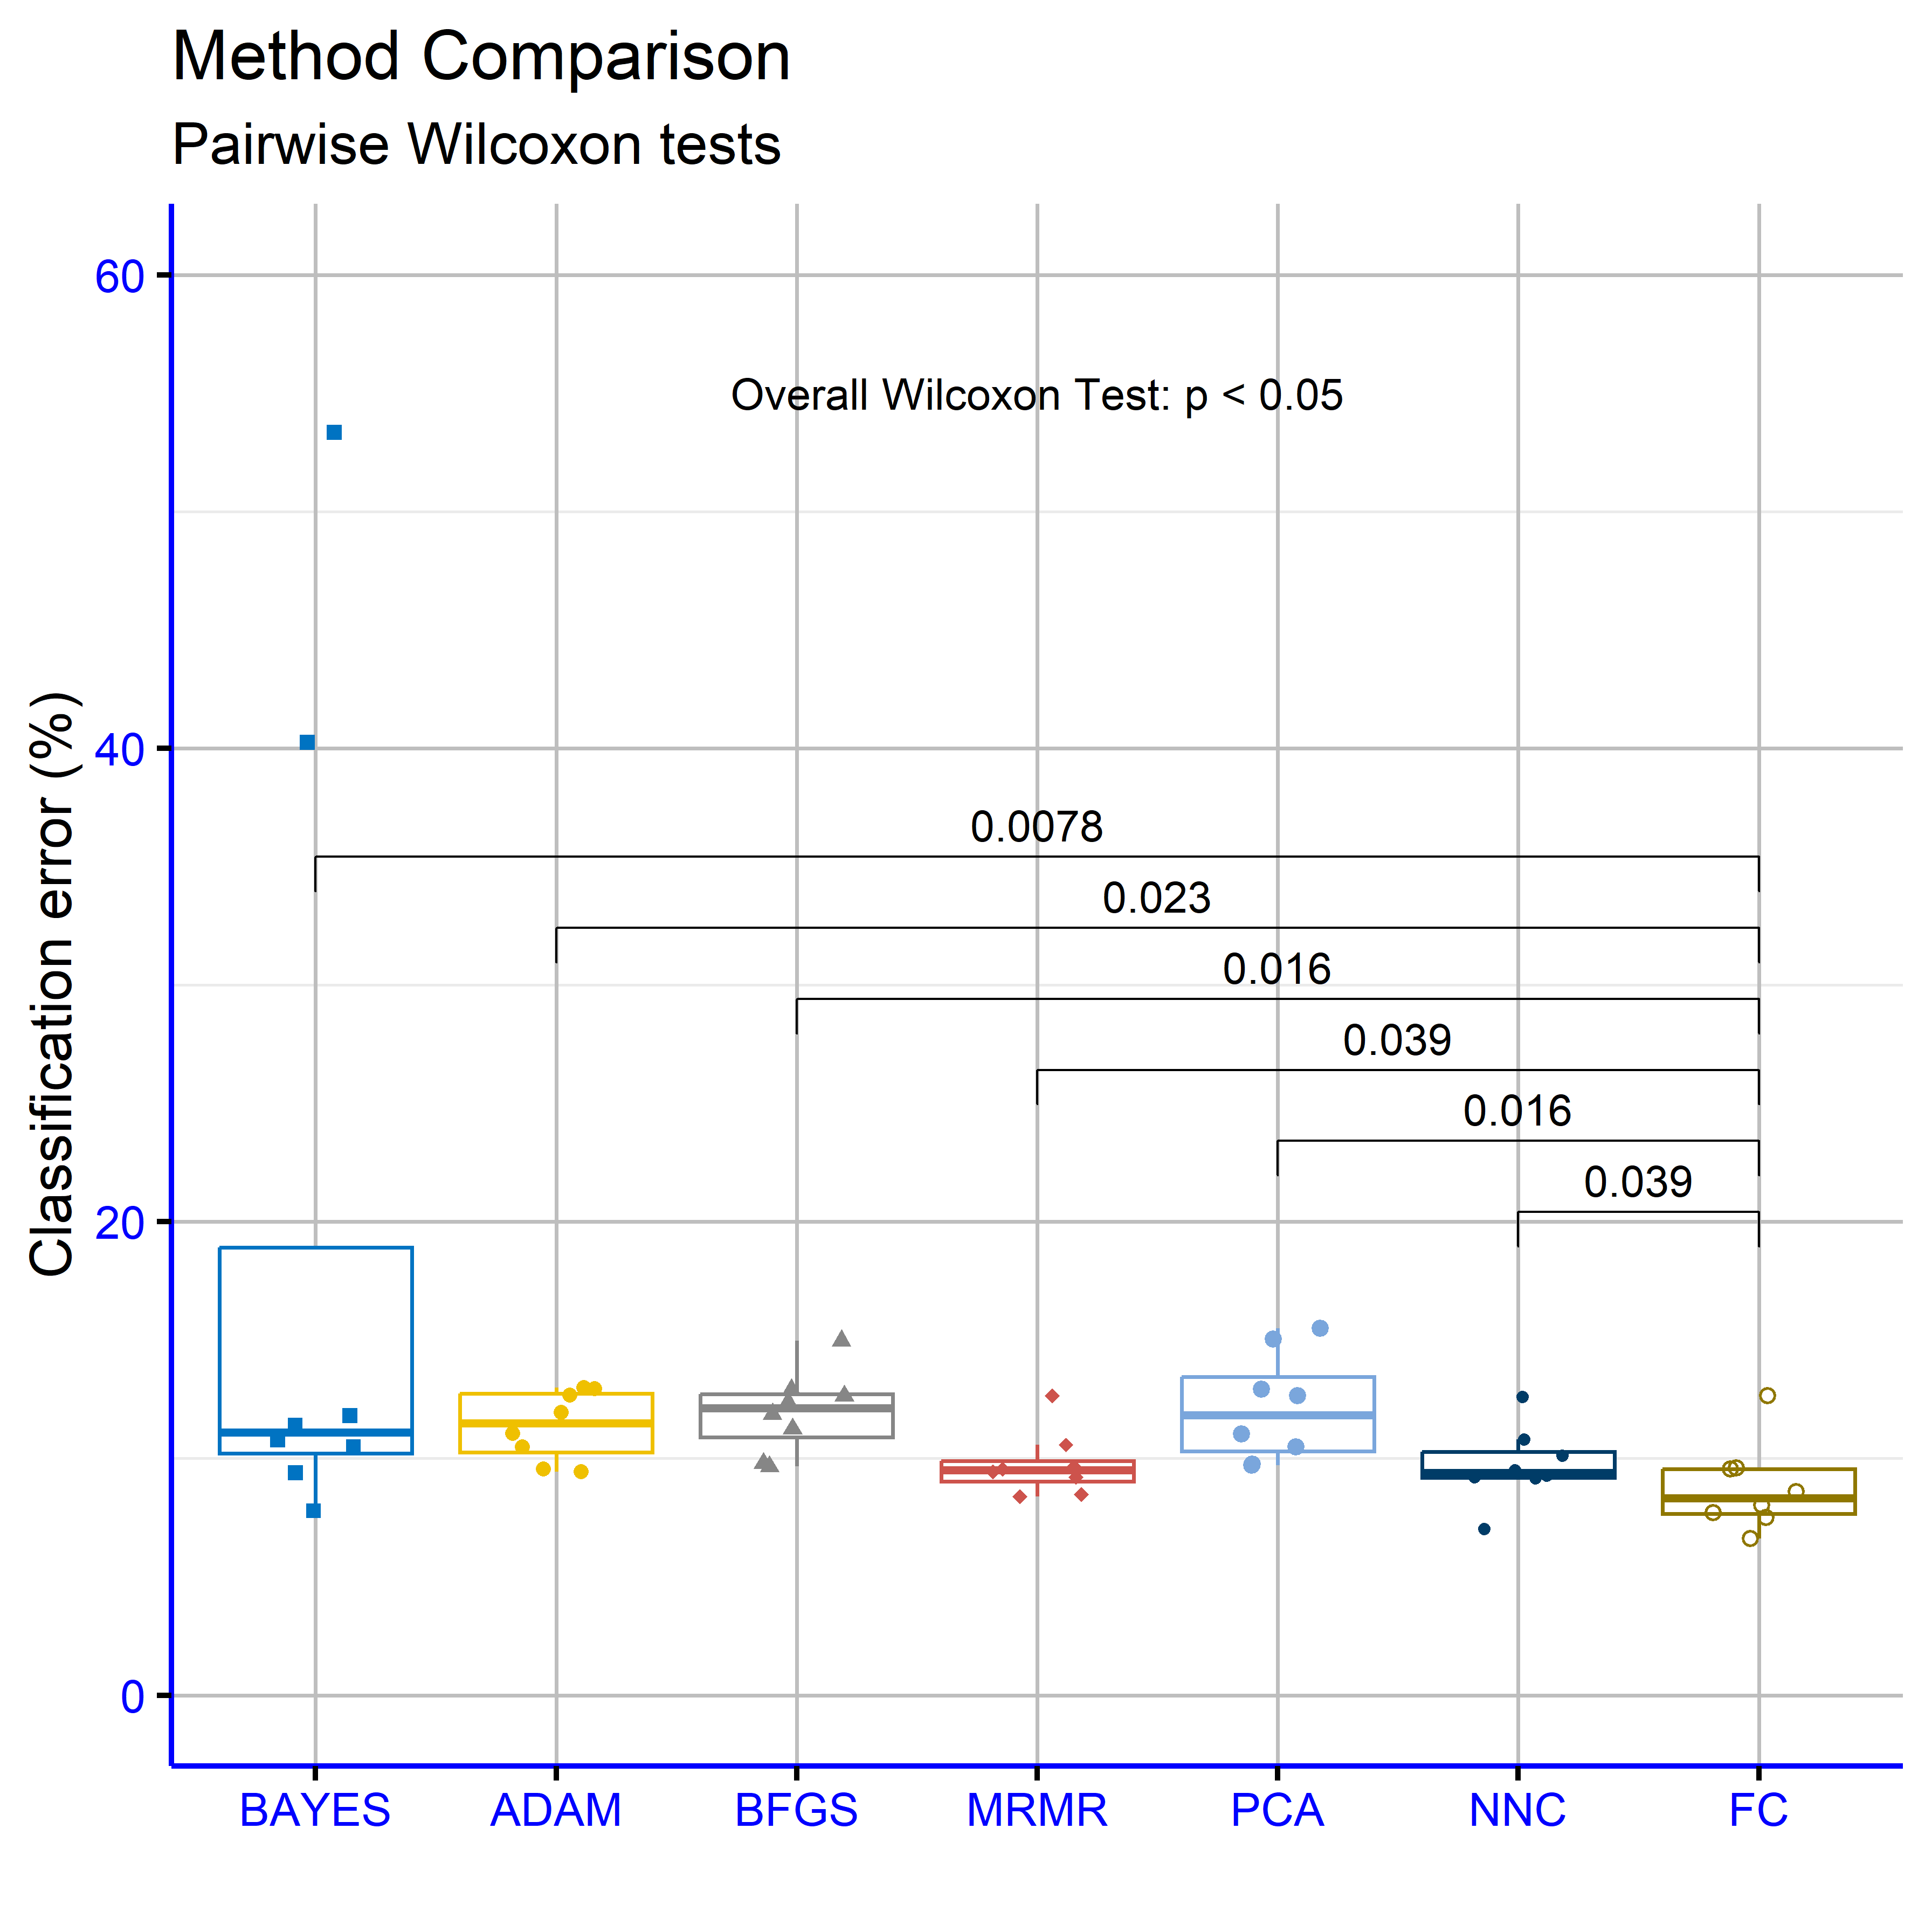
\includegraphics[scale=0.5]{statWilcoxon}

\caption{Statistical comparison of the used machine learning techniques.\label{fig:statExper}}

\end{figure}
The data in Table \ref{tab:experNF} present the classification error
rates for the \textquotedbl FC\textquotedbl{} machine learning model
across different numbers of constructed features ($N_{f}=1$, $N_{f}=2$,
and $N_{f}=3$) generated using Grammatical Evolution, spanning the
years 2014 to 2021. These results provide insights into the impact
of the number of features on the model's performance over time. For
$N_{f}=1$, the classification error rates exhibit variability across
the years, ranging from a minimum of 6.77\% in 2019 to a maximum of
12.68\% in 2017. The average error rate for this configuration is
9.03\%, indicating a relatively moderate level of accuracy overall.
The peak error in 2017 suggests possible challenges in that year's
data or specific interactions between the model and the constructed
feature set. For $N_{f}=2$, the classification error rates show a
slightly improved overall performance compared to $N_{f}=1$, with
an average error of 8.79\%. The error rates range from 6.62\% in 2019,
marking the lowest rate for this configuration, to 12.66\% in 2017,
the highest. These results indicate that adding one more feature generally
leads to improved accuracy, although the improvement is not uniform
across all years. For $N_{f}=3$, the classification error rates demonstrate
further improvement, with an average error of 8.63\%, which is the
lowest among the three configurations. The error rates range from
a minimum of 6.49\% in 2019 to a maximum of 12.46\% in 2017. The slightly
lower peak error compared to $N_{f}=1$ and $N_{f}=2$ suggests that
the inclusion of a third constructed feature enhances the model's
ability to capture data patterns more effectively. Across all configurations,
the year 2017 consistently exhibits the highest classification error
rates, irrespective of the number of features. This outlier suggests
specific data-related challenges or unique model behavior during that
year. Conversely, 2019 consistently shows the lowest error rates,
indicating favorable conditions for accurate classification during
that period. The trend in the average classification error rates decreasing
from 9.03\% for $N_{f}=1$ to 8.63\% for $N_{f}=3$ demonstrates that
the addition of constructed features through Grammatical Evolution
positively impacts the model's accuracy. However, the diminishing
returns between $N_{f}=2$ and $N_{f}=3$ suggest that the incremental
benefit of adding more features may plateau after a certain point.
In conclusion, the analysis reveals that increasing the number of
constructed features generally improves the accuracy of the \textquotedbl FC\textquotedbl{}
model. The results highlight the importance of balancing feature complexity
and model performance while considering the specific characteristics
of the data across different years.

\begin{table}[H]

\caption{Experiments with different number of constructed features for the
procedure that creates artificial features with Grammatical Evolution.\label{tab:experNF}}

\centering{}%
\begin{tabular}{|c|c|c|c|}
\hline 
YEAR & $N_{f}=1$ & $N_{f}=2$ & $N_{f}=3$\tabularnewline
\hline 
\hline 
2014 & 8.36\% & 8.04\% & 7.95\%\tabularnewline
\hline 
2015 & 8.10\% & 7.51\% & 7.24\%\tabularnewline
\hline 
2016 & 8.61\% & 8.60\% & 8.15\%\tabularnewline
\hline 
2017 & 12.68\% & 12.66\% & 12.46\%\tabularnewline
\hline 
2018 & 7.68\% & 7.72\% & 7.51\%\tabularnewline
\hline 
2019 & 6.77\% & 6.62\% & 6.49\%\tabularnewline
\hline 
2020 & 9.50\% & 9.61\% & 9.58\%\tabularnewline
\hline 
2021 & 10.53\% & 9.55\% & 9.62\%\tabularnewline
\hline 
\textbf{AVERAGE} & \textbf{9.03\%} & \textbf{8.79\%} & \textbf{8.63\%}\tabularnewline
\hline 
\end{tabular}
\end{table}
For Table \ref{tab:experNF}, a statistical analysis was conducted
using the Wilcoxon Test (Figure \ref{fig:statNf}) to compare classification
error rates among configurations with different numbers of constructed
features ($N_{f}=1,N_{f}=2$, and $N_{f}=3$). The results of the
test provide valuable insights into the statistical significance of
the differences in the performance of these configurations. The overall
result of the Wilcoxon Test, with p \textless{} 0.5, indicates that
statistically significant differences exist in at least one of the
pairwise comparisons between the configurations. Specifically, the
comparison between $N_{f}=1$ and $N_{f}=2$ yields p = 0.15, which
is not statistically significant. This suggests that adding a second
constructed feature does not lead to a significant improvement in
the model’s performance. On the other hand, the comparison between
$N_{f}=1$ and $N_{f}=3$ shows p = 0.016, a statistically significant
value. This indicates that the inclusion of a third constructed feature
substantially enhances the model’s accuracy compared to using only
one feature. The comparison between $N_{f}=2$ and $N_{f}=3$ also
reveals a statistically significant difference, with p = 0.023. This
result suggests that even the transition from $N_{f}=2$ to $N_{f}=3$
leads to an improvement in performance, although the difference is
less pronounced than between $N_{f}=1$ and $N_{f}=3$. Overall, the
analysis demonstrates that increasing the number of constructed features
from $N_{f}=1$ to $N_{f}=3$ results in a statistically significant
improvement in the model’s accuracy. The comparison between $N_{f}=1$
and $N_{f}=2$ is not statistically significant, possibly due to the
limited impact of adding only one additional feature. In contrast,
the difference between $N_{f}=2$ and $N_{f}=3$ highlights that further
increasing the number of features continues to enhance performance,
albeit to a lesser degree.
\begin{figure}[H]
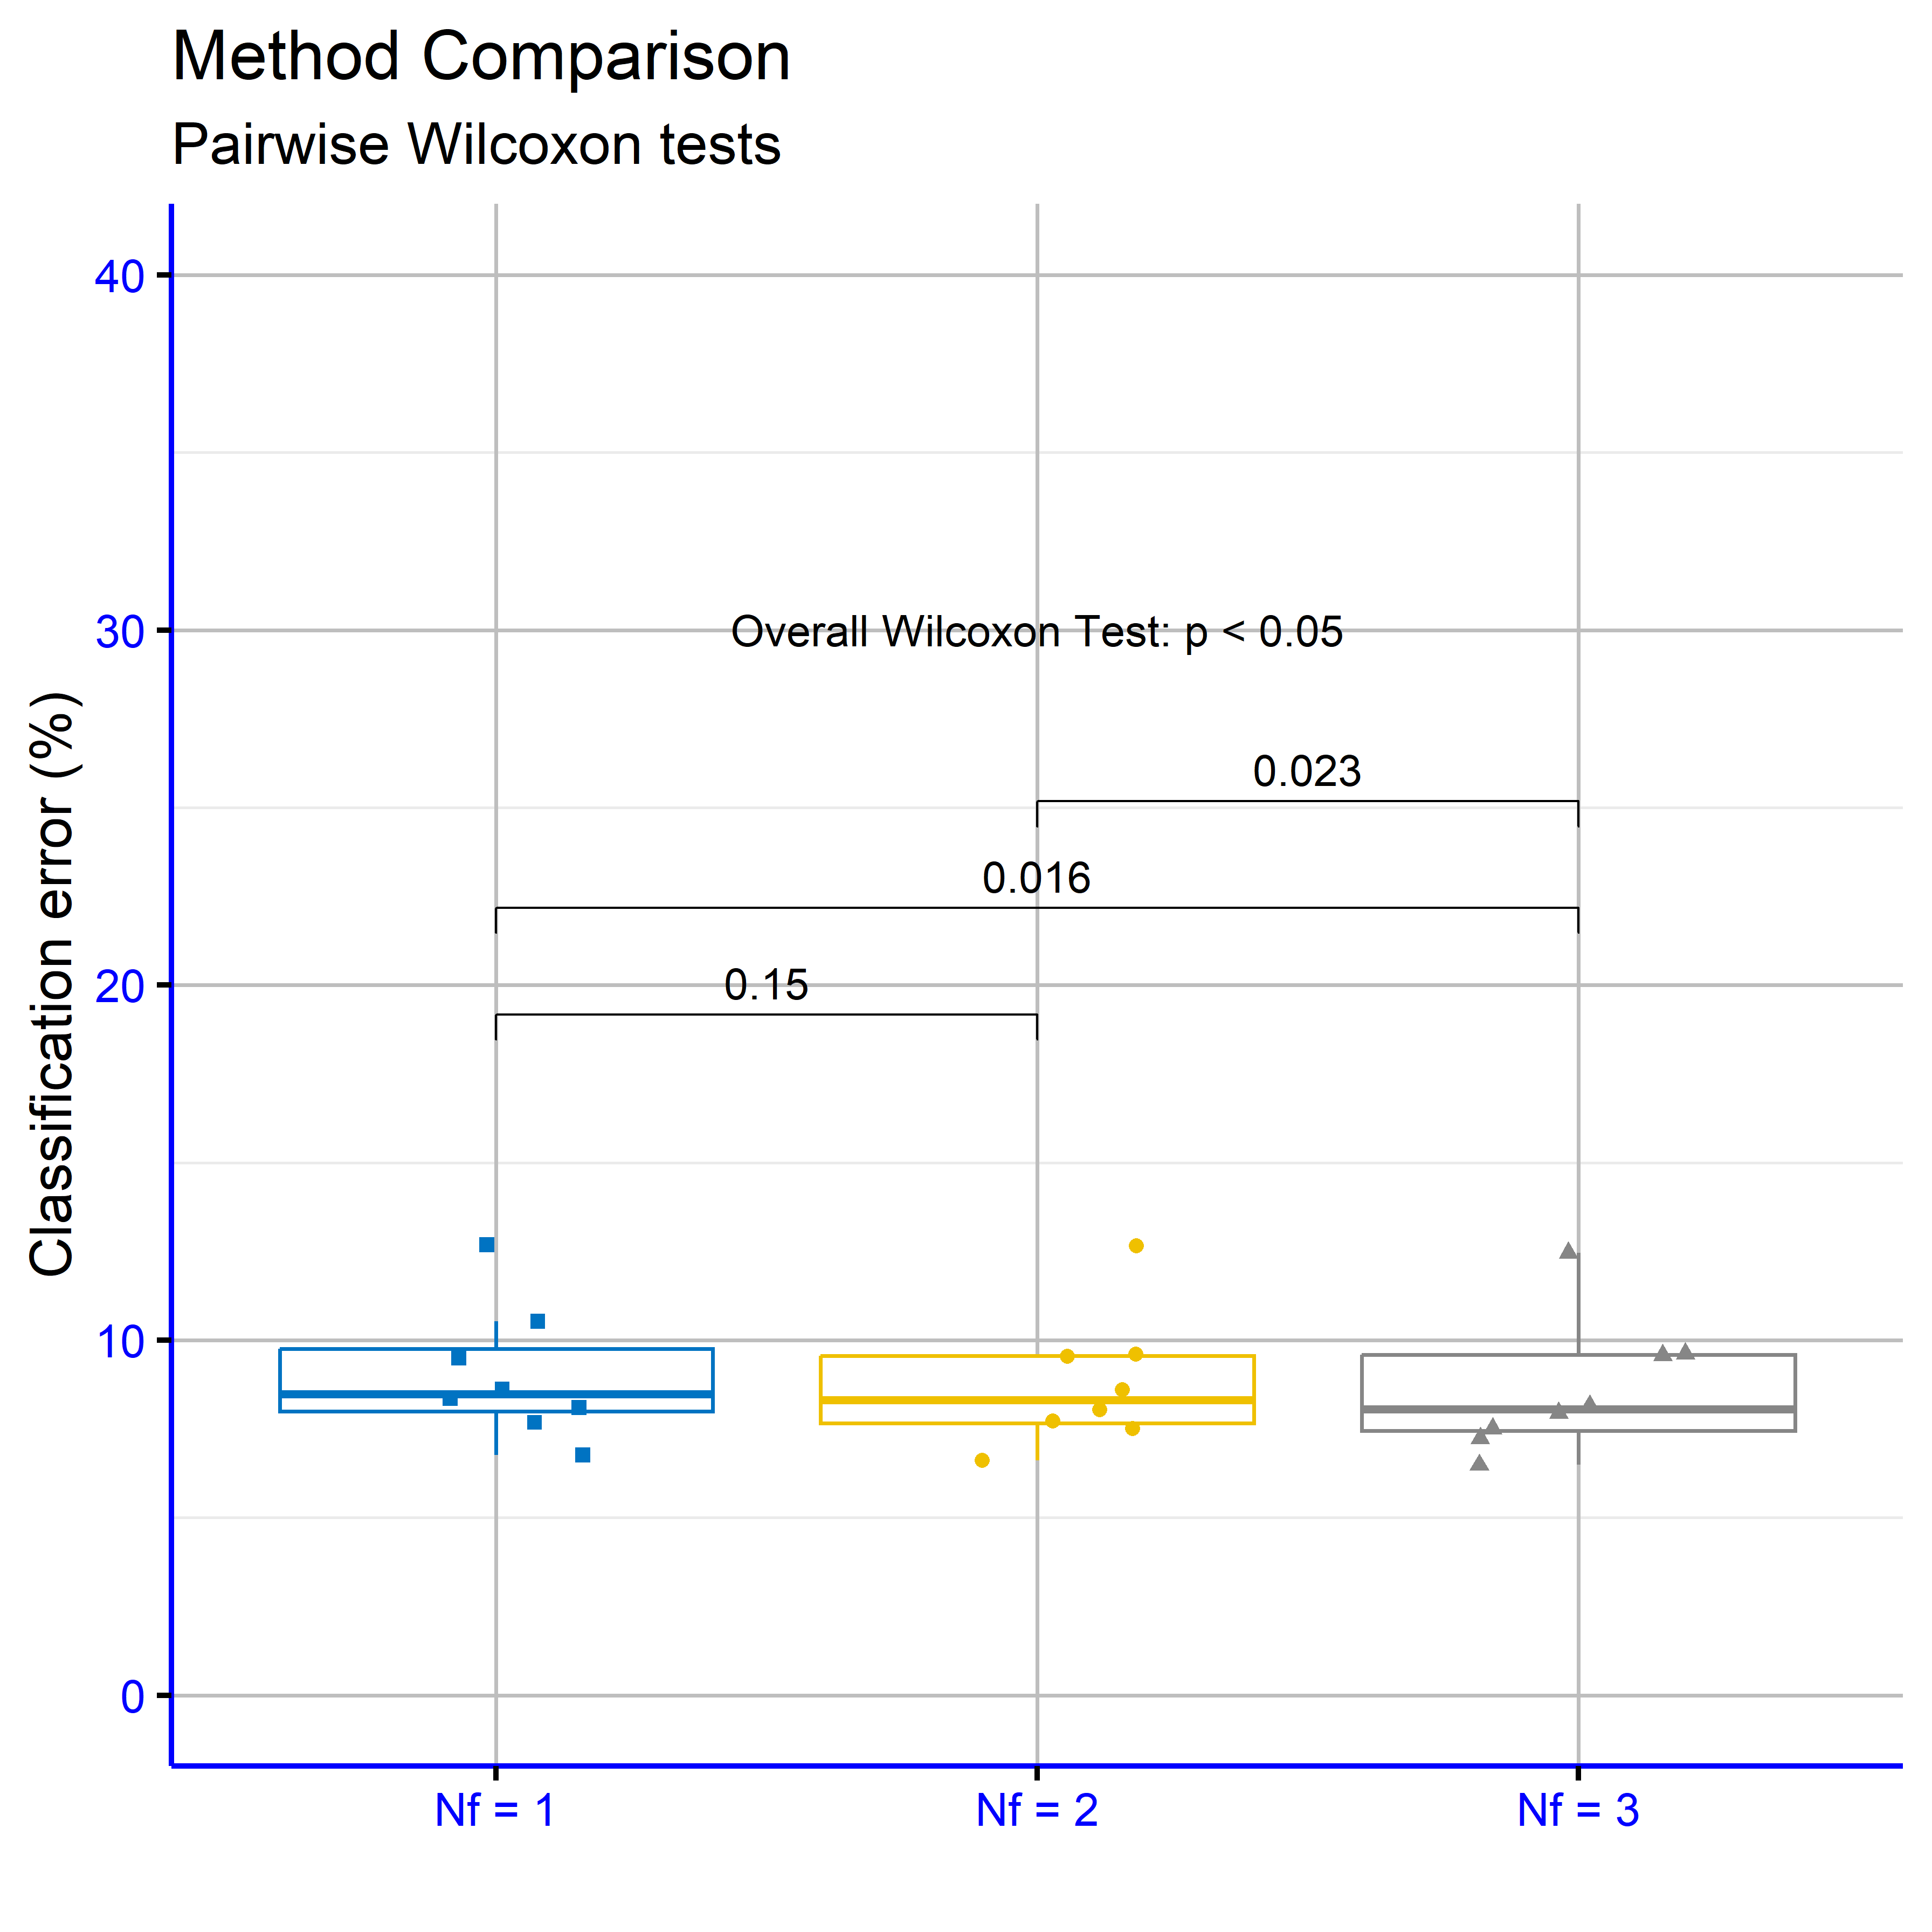
\includegraphics[scale=0.5]{statWilcoxon2}

\caption{Statistical comparison for the experiment involving different values
of the critical parameter $N_{f}$.\label{fig:statNf}}

\end{figure}


\section{Conclusions\label{sec:Conclusions}}

The study examines the application of feature construction techniques
for predicting the duration of forest fires using data collected in
Greece over a ten-year period. The methods utilized include Principal
Component Analysis (PCA), Minimum Redundancy Maximum Relevance (MRMR),
and Grammatical Evolution for constructing artificial features and
generating neural networks. The analysis focused on meteorological
parameters such as temperature, humidity, wind, and rainfall, which
significantly influence the behavior of forest fires. The research
concluded that the feature construction technique, using grammatical
evolution, outperforms other methods in terms of stability and accuracy.
The results indicated that this technique achieved the lowest error
rate in predicting fire duration compared to other approaches such
as PCA, MRMR, and traditional algorithms like Bayes and Adam. While
PCA proved effective for dimensionality reduction, it often led to
a loss of critical information. MRMR, though capable of identifying
relevant features, did not exhibit consistent performance across all
datasets. Traditional algorithms like Bayes showed significant variability,
with their performance heavily influenced by the data characteristics.
Statistical analysis using the Wilcoxon test demonstrated the clear
superiority of feature construction over other methods. This advantage
can be attributed to the technique's ability to adapt to the peculiarities
of the data, avoiding the information loss observed with other approaches.
Specifically, the method excelled in both accuracy and robustness.
The study's findings underscore the potential of advanced machine
learning techniques in addressing critical environmental challenges
such as forest fires. Future research could focus on integrating data
from diverse geographical regions or climatic conditions, developing
automated real-time monitoring systems, and combining advanced algorithms
for even more efficient analysis. Incorporating social and environmental
factors into predictive models could also offer a multidimensional
understanding of the causes and spread of fires. Overall, this study
highlights the importance of scientific approaches and technology
in tackling contemporary challenges posed by climate change and natural
disasters.

\vspace{6pt}


\authorcontributions{C.K., V.C.,A.M. and I.G.T. conceived of the idea and the methodology,
and C.K. and V.C. implemented the corresponding software. C.K. and
A.M. conducted the experiments, employing objective functions as test
cases, and provided the comparative experiments. V.C. performed the
necessary statistical tests. All authors have read and agreed to the
published version of the manuscript.}

\funding{This research received no external funding.}

\institutionalreview{Not applicable. }

\informedconsent{Not applicable. }

\dataavailability{Not applicable. }

\acknowledgments{This research has been financed by the European Union: Next Generation
EU through the Program Greece 2.0 National Recovery and Resilience
Plan, under the call RESEARCH--CREATE--INNOVATE, project name “iCREW:
Intelligent small craft simulator for advanced crew training using
Virtual Reality techniques” (project code: TAEDK-06195).}

\conflictsofinterest{The authors declare no conflicts of interest.}

\appendixtitles{no}

\begin{adjustwidth}{-\extralength}{0cm}{}


\reftitle{References}
\begin{thebibliography}{999}
\bibitem[(2017)]{Field } Field, J. F. (2017). London, Londoners and
the Great Fire of 1666: disaster and recovery. Routledge.

\bibitem{fire1}Gowlett, J.A.J. The discovery of fire by humans: a
long and convoluted process. Philosophical Transaction B, Biological
Sciences, volume 371, Issue 1696. June 5, 2016.

\bibitem{fire2}Heinonen, Keri. The Fire of Prometheus: More Than
Just a Gift to Humanity. Greek Mythology. November 19, 2024. Available
from: https://greek.mythologyworldwide.com/the-fire-of-prometheus-more-than-just-a-gift-to-humanity/
(accessed on November 29, 2024).

\bibitem{fire3}McCaffrey, S. (2004). Thinking of wildfire as a natural
hazard. Society and Natural Resources, 17(6), 509-516.

\bibitem{fire4}Patrick, Van Hees. The burning challenge of fire safety.
ISO, International Organization for Standardization. Available from:
https://www.iso.org/news/2014/11/Ref1906.html (accessed on December
3, 2024).

\bibitem{fire5}UNEP. United Nations Environment Programme. Number
of wildfires to rise by 50 per cent by 2100 and governments are not
prepared, experts warn. 23 February 2022. Available from: https://www.unep.org/news-and-stories/press-release/number-wildfires-rise-50-cent-2100-and-governments-are-not-prepared
(accessed on December 4, 2024).

\bibitem{fire_nasa}NASA. Carbon Dioxide, Vital Signs. October 2024.
Available from: https://climate.nasa.gov/vital-signs/carbon-dioxide/?intent=121
(accessed on November 29, 2024). 

\bibitem{fire_iliopoulos}Iliopoulos, N., Aliferis, I., \& Chalaris,
M. (2024). Effect of Climate Evolution on the Dynamics of the Wildfires
in Greece. Fire, 7(5), 162.

\bibitem{fire_giorgi}Giorgi, F. (2006). Climate change hot‐spots.
Geophysical research letters, 33(8).

\bibitem{ai_climate}Satish, M., Prakash., Babu, S.M., Kumar, P.P.,
Devi, S., Reddy, K.P. Artificial Intelligence (AI) and the Prediction
of Climate Change Impacts. 2023. IEEE 5th International Conference
on Cybernetics, Cognition and Machine Learning Applications (ICCCMLA).

\bibitem{ai_ml}Walsh, Dylan. Tackling climate change with machine
learning. MIT Management Sloan School. Climate Change. October 24,
2023. Available from: https://mitsloan.mit.edu/ideas-made-to-matter/tackling-climate-change-machine-learning
(accessed on November 29, 2024). 

\bibitem{iso_ml}ISO. Machine Learning (ML): All there is to know.
International Organization for Standardization. Available from: https://www.iso.org/artificial-intelligence/machine-learning
(accessed on November 30, 2024).

\bibitem{ml_turing}Watson, Ian. (2012). How Alan Turing Invented
the Computer Age. Scientific American. Published: 26/04/2012.Available
from: https://blogs.scientificamerican.com/guest-blog/how-alan-turing-invented-the-computer-age/
(accessed on November 30, 2024). 

\bibitem{ml_review}Jain, P., Coogan, S. C., Subramanian, S. G., Crowley,
M., Taylor, S., \& Flannigan, M. D. (2020). A review of machine learning
applications in wildfire science and management. Environmental Reviews,
28(4), 478-505.

\bibitem{fire_manage}Xiao, H. (2023). Estimating fire duration using
regression methods. arXiv preprint arXiv:2308.08936.

\bibitem{fire_manage2}Linardos, V., Drakaki, M., Tzionas, P., \&
Karnavas, Y. L. (2022). Machine learning in disaster management: recent
developments in methods and applications. Machine Learning and Knowledge
Extraction, 4(2).

\bibitem{fire_bayes1}Sevinc, V., Kucuk, O., \& Goltas, M. (2020).
A Bayesian network model for prediction and analysis of possible forest
fire causes. Forest Ecology and Management, 457, 117723.

\bibitem{fire_bayes2}Chen, F., Jia, H., Du, E., Chen, Y., \& Wang,
L. (2024). Modeling of the cascading impacts of drought and forest
fire based on a Bayesian network. International Journal of Disaster
Risk Reduction, 111, 104716.

\bibitem{fire_bayes3}Kim, B., \& Lee, J. (2021). A Bayesian network-based
information fusion combined with DNNs for robust video fire detection.
Applied Sciences, 11(16), 7624.

\bibitem{fire_naive1}Nugroho, A. A., Iwan, I., Azizah, K. I. N.,
\& Raswa, F. H. (2019). Peatland Forest Fire Prevention Using Wireless
Sensor Network Based on Naïve Bayes Classifier. KnE Social Sciences,
20-34.

\bibitem{fire_naive2}Zainul, M., \& Minggu, E. (2022). Classification
of Hotspots Causing Forest and Land Fires Using the Naive Bayes Algorithm.
Interdisciplinary Social Studies, 1(5), 555-567.

\bibitem{fire_naive3}Karo, I. M. K., Amalia, S. N., \& Septiana,
D. Wildfires Classification Using Feature Selection with K-NN, Naïve
Bayes, and ID3 Algorithms. Journal of Software Engineering, Information
and Communication Technology (SEICT), 3(1), 15-24.

\bibitem{fire_log1}Vilar del Hoyo, L., Martín Isabel, M. P., \& Martínez
Vega, F. J. (2011). Logistic regression models for human-caused wildfire
risk estimation: analysing the effect of the spatial accuracy in fire
occurrence data. European Journal of Forest Research, 130, 983-996.

\bibitem{fire_log2}de Bem, P. P., de Carvalho Júnior, O. A., Matricardi,
E. A. T., Guimarães, R. F., \& Gomes, R. A. T. (2018). Predicting
wildfire vulnerability using logistic regression and artificial neural
networks: a case study in Brazil’s Federal District. International
journal of wildland fire, 28(1), 35-45.

\bibitem{fire_log3}Nhongo, E. J. S., Fontana, D. C., Guasselli, L.
A., \& Bremm, C. (2019). Probabilistic modelling of wildfire occurrence
based on logistic regression, Niassa Reserve, Mozambique. Geomatics,
Natural Hazards and Risk, 10(1), 1772-1792.

\bibitem{fire_log4}Peng, W., Wei, Y., Chen, G., Lu, G., Ye, Q., Ding,
R. \& Cheng, Z. (2023). Analysis of Wildfire Danger Level Using Logistic
Regression Model in Sichuan Province, China. Forests, 14(12), 2352.

\bibitem{fire_ann1}Hossain, F. A., Zhang, Y., Yuan, C., \& Su, C.
Y. (2019, July). Wildfire flame and smoke detection using static image
features and artificial neural network. In 2019 1st international
conference on industrial artificial intelligence (iai) (pp. 1-6).
IEEE.

\bibitem{fire_ann2}Lall, S., \& Mathibela, B. (2016, December). The
application of artificial neural networks for wildfire risk prediction.
In 2016 International Conference on Robotics and Automation for Humanitarian
Applications (RAHA) (pp. 1-6). IEEE.

\bibitem{fire_ann3}Sayad, Y. O., Mousannif, H., \& Al Moatassime,
H. (2019). Predictive modeling of wildfires: A new dataset and machine
learning approach. Fire safety journal, 104, 130-146.

\bibitem{fire_ann4}Gao, K., Feng, Z., \& Wang, S. (2022). Using multilayer
perceptron to predict forest fires in jiangxi province, southeast
china. Discrete Dynamics in Nature and Society, 2022(1), 6930812.

\bibitem{fire_rf1}Latifah, A. L., Shabrina, A., Wahyuni, I. N., \&
Sadikin, R. (2019, October). Evaluation of Random Forest model for
forest fire prediction based on climatology over Borneo. In 2019 International
Conference on Computer, Control, Informatics and its Applications
(IC3INA) (pp. 4-8). IEEE.

\bibitem{fire_rf2}Malik, A., Rao, M. R., Puppala, N., Koouri, P.,
Thota, V. A. K., Liu, Q., ... \& Gao, J. (2021). Data-driven wildfire
risk prediction in northern California. Atmosphere, 12(1), 109.

\bibitem[(2025)]{Song} Song, S., Zhou, X., Yuan, S., Cheng, P., \&
Liu, X. (2025). Interpretable artificial intelligence models for predicting
lightning prone to inducing forest fires. Journal of Atmospheric and
Solar-Terrestrial Physics, 267, 106408.

\bibitem{fire_rf3}Gao, C., Lin, H., \& Hu, H. (2023). Forest-fire-risk
prediction based on random forest and backpropagation neural network
of Heihe area in Heilongjiang province, China. Forests, 14(2), 170.

\bibitem[(2025)]{Hu} Hu, Z., Zhao, J., Zhang, S., Ma, H., \& Zhang,
J. (2025). Development and Validation of a Novel Method to Predict
Flame Behavior in Tank Fires Based on CFD Modeling and Machine Learning.
Reliability Engineering \& System Safety, 111368. 

\bibitem{duration_andela}Andela, N., Morton, D. C., Giglio, L., Paugam,
R., Chen, Y., Hantson, S. \& Randerson, J. T. (2019). The Global Fire
Atlas of individual fire size, duration, speed and direction. Earth
System Science Data, 11(2), 529-552.

\bibitem{duration_surrogate}Kc, U., Aryal, J., Hilton, J., \& Garg,
S. (2021). A surrogate model for rapidly assessing the size of a wildfire
over time. Fire, 4(2), 20.

\bibitem{key-2} Xie, Zi-Cong and Xu, Zhao-Dong and Gai, Pan-Pan and
Xia, Zhi-Heng and Xu, Ye-Shou. (2025). A deep learning-{}-based surrogate
model for spatial-temporal temperature field prediction in subway
tunnel fires via CFD simulation. Journal of Dynamic Disasters, 1,1,pp.
100002. 

\bibitem{duration_wang}Liang, H., Zhang, M., \& Wang, H. (2019).
A neural network model for wildfire scale prediction using meteorological
factors. IEEE Access, 7, 176746-176755.

\bibitem[(2025)]{Zhai} Zhai, X., Kong, W., Hu, Z., Zhang, C., Ma,
H., \& Zhao, J. (2025). Prediction method and application of temperature
distribution in typical confined space spill fires based on deep learning.
Process Safety and Environmental Protection, 198, 107127.

\bibitem{duration_xi}Xi, D. D., Dean, C. B., \& Taylor, S. W. (2021).
Modeling the duration and size of wildfires using joint mixture models.
Environmetrics, 32(6), e2685.

\bibitem{duration_wfca}WFCA. Western Fire Chiefs Association. How
Long Do Wildfires Last? October 2022. Available from: https://wfca.com/wildfire-articles/how-long-do-wildfires-last/
(accessed on December 4, 2024). 

\bibitem{genfc1}M.G. Smith, L. Bull, Genetic Programming with a Genetic
Algorithm for Feature Construction and Selection, Genet Program Evolvable
Mach \textbf{6}, pp. 265--281, 2005.

\bibitem{pca1}A. Maćkiewicz, W. Ratajczak, Principal components analysis
(PCA). Computers \& Geosciences \textbf{19}, pp. 303-342, 1993.

\bibitem{pca_cadima}J. Cadima, I.T. Jolliffe, Principal component
analysis: a review and recent developments, National Library of Medicine.
2016. Available online: https://pmc.ncbi.nlm.nih.gov/articles/PMC4792409/
(accessed on 16 November 2024). 

\bibitem{pca_i2}i2tutorials. What are the Pros and Cons of the PCA?
October 1st, 2019. Available online: https://www.i2tutorials.com/what-are-the-pros-and-cons-of-the-pca/
(accessed on 16 November 2024). 

\bibitem{pca_park}S.C. Park, Physical Meaning of Principal Component
Analysis for Lattice Systems with Translational Invariance. arXiv
preprint arXiv:2410.22682, 2024.

\bibitem{pca_sarma}O. Sarma, M.A. Rather, S. Shahnaz, R.S. Barwal,
Principal Component Analysis of Morphometric Traits in Kashmir Merino
Sheep. Journal of Advances in Biology \& Biotechnology \textbf{27},
pp. 362-69, 2024.

\bibitem{pca_parente}C. Gambardella, R. Parente, A. Ciambrone, M.
Casbarra, A Principal Components Analysis -- Based Method for the
Detection of Cannabis Plants Using Representation data by Remote Sensing,
Knowledge Extractions from data Using Machine Learning, volume 6 (10),
2021.

\bibitem{pca_electric}M. Slavkovic, D. Jevtic, Face Recognition Using
Eigenface Approach, Serbian Journal of Electrical Engineering \textbf{9},
pp. 121-130, 2012.

\bibitem{pca_stock}C.A. Hargreaves, C.K. Mani, The Selection of Winning
Stocks Using Principal Component Analysis, American Journal of Marketing
Research \textbf{1}, pp. 183 -- 188, 2015.

\bibitem{pca_kernel}Z. Xu, F. Guo, H. Ma, X. Liu, L. Gao, On Optimizing
Hyperspectral Inversion of Soil Copper Content by Kernel Principal
Component Analysis. Remote Sensing \textbf{16}, 2024.

\bibitem{pca_zhang}H. Zhang, R. Srinivasa, X. Yang, S. Ahrentzen,
E.S. Coker, A. Alwisy, Factors influencing indoor air pollution in
buildings using PCA -- LMBP neural network: A case study of a university
campus, Building and environment \textbf{225}, 2022.

\bibitem{lm_paper}M.I. Lourakis, A brief description of the Levenberg-Marquardt
algorithm implemented by levmar, Foundation of Research and Technology
\textbf{4}, pp. 1-6, 2005.

\bibitem{pca_svm}B.A. Akinnuwesi, B.O. Macaulay, B.S. Aribisala,
Breast cancer risk assessment and early diagnosis using Principal
Component Analysis and support vector machine techniques, Informatics
in medicine unlocked \textbf{21}, 100459, 2020.

\bibitem{svm}M. Awad, R. Khanna, M. Awad, R. Khanna, Support vector
machines for classification. Efficient learning machines: Theories,
concepts, and applications for engineers and system designers, pp.
39-66, 2015.

\bibitem{pca_guan}R. Guan, Predicting forest fire with linear regression
and random forest, Highlights in Science, Engineering and Technology
\textbf{44}, pp. 1-7, 2023.

\bibitem{pca_nikolov}N. Nikolov, P. Bothwell, J. Snook, Developing
a gridded model for probabilistic forecasting of wildland-fire ignitions
across the lower 48 States. USFS-CSU Joint Venture Agreement Phase
2 (2019-2021)-Final Report. Fort Collins, CO: US Department of Agriculture,
Forest Service, Rocky Mountain Research Station. 33p, 2022.

\bibitem{pca_nikolov2}N. Nikolov, P. Bothwell, J. Snook, Probalistic
forecasting of lightning strikes over the Continental USA and Alaska:
Model development and verification. Scientific Journal, Fire (7).
Available from: https://research.fs.usda.gov/treesearch/68447 (accessed
20 November 2024). 

\bibitem[Author1(year)]{mrmr1} C. Ding, H. Peng, Minimum redundancy
feature selection from microarray gene expression data. Journal of
bioinformatics and computational biology \textbf{3}, pp. 185-205,
2005.

\bibitem{mrmr2}S. Ramirez -- Gallego, I. Lastra, D. Martinez --
Rego, V. Bolon -- Canedo, J.M. Benitez, F. Herrera, A. Alonso --
Betanzos, Fast-mRMR: Fast Minimum Redundancy Maximum Relevance Algorithm
for High -- Dimensional Big Data, International Journal of Intelligent
Systems \textbf{32}, pp. 134 -- 152, 2017.

\bibitem{mrmr_zhao}Zhao, Z., Anand, R., \& Wang, M. (2019, October).
Maximum relevance and minimum redundancy feature selection methods
for a marketing machine learning platform. In 2019 IEEE international
conference on data science and advanced analytics (DSAA) (pp. 442-452).
IEEE.

\bibitem{random_forest}S.J. Rigatti, Random forest. Journal of Insurance
Medicine \textbf{47}, pp. 31-39, 2017.

\bibitem{mrmr_wu}Wu, H., Yang, T., Li, H., \& Zhou, Z. (2023). Air
quality prediction model based on mRMR--RF feature selection and
ISSA--LSTM. Scientific Reports, 13(1), 12825.

\bibitem{mrmr_elbeltagi}Elbeltagi, A., Nagy, A., Szabo, A., Nxumalo,
G.S., Bodi, E.B., Tamas, J. Hyperspectral indices data fusion-based
machine learning enhanced by MRMR algorithm for estimating maize chlorophyll
content. Frontiers in Plant Science, Section Technical Advances in
Plant Science, volume 15, October 2024. 

\bibitem{mrmr_liu}Liu, J., Sun, H., Li, Y., Fang, W., \& Niu, S.
(2020). An improved power system transient stability prediction model
based on mRMR feature selection and WTA ensemble learning. Applied
Sciences, 10(7), 2255.

\bibitem{eml}Dietterich, T. G. (2000, June). Ensemble methods in
machine learning. In International workshop on multiple classifier
systems (pp. 1-15). Berlin, Heidelberg: Springer Berlin Heidelberg.

\bibitem{mrmr_eristi}Eristi, B. (2024). A New Approach based on Deep
Features of Convolutional Neural Networks for Partial Discharge Detection
in Power Systems. IEEE Access.

\bibitem{mrmr_zhang}Li, Y., Zhang, Y., Zhu, H., Yan, R., Liu, Y.,
Sun, L., \& Zeng, Z. (2015). Recognition algorithm of acoustic emission
signals based on conditional random field model in storage tank floor
inspection using inner detector. Shock and Vibration, 2015(1), 173470.

\bibitem{mrmr_razmi}Karamouz, M., Zahmatkesh, Z., Nazif, S., \& Razmi,
A. (2014). An evaluation of climate change impacts on extreme sea
level variability: Coastal area of New York City. Water resources
management, 28, 3697-3714.

\bibitem{ge1}M. O’Neill, C. Ryan, Grammatical evolution, IEEE Trans.
Evol. Comput. \textbf{5,}pp. 349--358, 2001.

\bibitem{nnc}I.G. Tsoulos, D. Gavrilis, E. Glavas, Neural network
construction and training using grammatical evolution, Neurocomputing
\textbf{72}, pp. 269-277, 2008.

\bibitem{nnc_amide1}G.V. Papamokos, I.G. Tsoulos, I.N. Demetropoulos,
E. Glavas, Location of amide I mode of vibration in computed data
utilizing constructed neural networks, Expert Systems with Applications
\textbf{36}, pp. 12210-12213, 2009.

\bibitem{nnc_de}I.G. Tsoulos, D. Gavrilis, E. Glavas, Solving differential
equations with constructed neural networks, Neurocomputing \textbf{72},
pp. 2385-2391, 2009.

\bibitem{nnc_feas}I.G. Tsoulos, G. Mitsi, A. Stavrakoudis, S. Papapetropoulos,
Application of Machine Learning in a Parkinson's Disease Digital Biomarker
Dataset Using Neural Network Construction (NNC) Methodology Discriminates
Patient Motor Status, Frontiers in ICT 6, 10, 2019.

\bibitem{nnc_student}V. Christou, I.G. Tsoulos, V. Loupas, A.T. Tzallas,
C. Gogos, P.S. Karvelis, N. Antoniadis, E. Glavas, N. Giannakeas,
Performance and early drop prediction for higher education students
using machine learning, Expert Systems with Applications \textbf{225},
120079, 2023.

\bibitem{nnc_autism}E.I. Toki, J. Pange, G. Tatsis, K. Plachouras,
I.G. Tsoulos, Utilizing Constructed Neural Networks for Autism Screening,
Applied Sciences \textbf{14}, 3053, 2024.

\bibitem{bnf1}J. W. Backus. The Syntax and Semantics of the Proposed
International Algebraic Language of the Zurich ACM-GAMM Conference.
Proceedings of the International Conference on Information Processing,
UNESCO, 1959, pp.125-132.

\bibitem{fc1}Dimitris Gavrilis, Ioannis G. Tsoulos, Evangelos Dermatas,
Selecting and constructing features using grammatical evolution, Pattern
Recognition Letters \textbf{29},pp. 1358-1365, 2008. 

\bibitem{fc2}Dimitris Gavrilis, Ioannis G. Tsoulos, Evangelos Dermatas,
Neural Recognition and Genetic Features Selection for Robust Detection
of E-Mail Spam, Advances in Artificial Intelligence Volume 3955 of
the series Lecture Notes in Computer Science pp 498-501, 2006.

\bibitem{fc3}George Georgoulas, Dimitris Gavrilis, Ioannis G. Tsoulos,
Chrysostomos Stylios, João Bernardes, Peter P. Groumpos, Novel approach
for fetal heart rate classification introducing grammatical evolution,
Biomedical Signal Processing and Control \textbf{2},pp. 69-79, 2007 

\bibitem{fc4}Otis Smart, Ioannis G. Tsoulos, Dimitris Gavrilis, George
Georgoulas, Grammatical evolution for features of epileptic oscillations
in clinical intracranial electroencephalograms, Expert Systems with
Applications \textbf{38}, pp. 9991-9999, 2011 

\bibitem{fc5}A. T. Tzallas, I. Tsoulos, M. G. Tsipouras, N. Giannakeas,
I. Androulidakis and E. Zaitseva, Classification of EEG signals using
feature creation produced by grammatical evolution, In: 24th Telecommunications
Forum (TELFOR), pp. 1-4, 2016.

\bibitem{rbf1}J. Park and I. W. Sandberg, Universal Approximation
Using Radial-Basis-Function Networks, Neural Computation 3, pp. 246-257,
1991.

\bibitem{rbf2}H. Yu, T. Xie, S. Paszczynski, B. M. Wilamowski, Advantages
of Radial Basis Function Networks for Dynamic System Design, in IEEE
Transactions on Industrial Electronics \textbf{58}, pp. 5438-5450,
2011.

\bibitem{nn1}C. Bishop, Neural Networks for Pattern Recognition,
Oxford University Press, 1995.

\bibitem{nn2}G. Cybenko, Approximation by superpositions of a sigmoidal
function, Mathematics of Control Signals and Systems \textbf{2}, pp.
303-314, 1989.

\bibitem{powell}M.J.D Powell, A Tolerant Algorithm for Linearly Constrained
Optimization Calculations, Mathematical Programming \textbf{45}, pp.
547-566, 1989.

\bibitem[(2025)]{optimus}I.G. Tsoulos, V. Charilogis, G. Kyrou, V.N.
Stavrou, A. Tzallas, Journal of Open Source Software \textbf{10},
7584, 2025.

\bibitem{weka_main}M. Hall, F. Frank, G. Holmes, B. Pfahringer, P.
Reutemann, I.H. Witten, The WEKA data mining software: an update.
ACM SIGKDD explorations newsletter \textbf{11}, pp. 10-18, 2009.

\bibitem{weka_education1}S.B. Aher, L.M.R.J. Lobo, Data mining in
educational system using weka. In International conference on emerging
technology trends, Foundation of Computer Science \textbf{3}, pp.
20-25, 2011.

\bibitem{weka_education2}S. Hussain, N.A. Dahan, F.M. Ba-Alwib, N.
Ribata, Educational data mining and analysis of students’ academic
performance using WEKA. Indonesian Journal of Electrical Engineering
and Computer Science \textbf{9}, pp. 447-459, 2018.

\bibitem{weka_medical1}A.K. Sigurdardottir, H. Jonsdottir, R. Benediktsson,
Outcomes of educational interventions in type 2 diabetes: WEKA data-mining
analysis. Patient education and counseling \textbf{67}, pp. 21-31,
2007.

\bibitem{weka_medical2}M.N. Amin, A. Habib, Comparison of different
classification techniques using WEKA for hematological data. American
Journal of Engineering Research \textbf{4}, pp. 55-61, 2015.

\bibitem{naive_bayes}G.I. Webb, E. Keogh, R. Miikkulainen, Naïve
Bayes, Encyclopedia of machine learning \textbf{15}, pp. 713-714,
2010.

\bibitem{nn_adam}D. P. Kingma, J. L. Ba, ADAM: a method for stochastic
optimization, in: Proceedings of the 3rd International Conference
on Learning Representations (ICLR 2015), pp. 1--15, 2015.

\bibitem{mlpack}Ryan R. Curtin, James R. Cline, N. P. Slagle, William
B. March, Parikshit Ram, Nishant A. Mehta, Alexander G. Gray, MLPACK:
A Scalable C++ Machine Learning Library, Journal of Machine Learning
Research \textbf{14}, pp. 801-805, 2013.

\bibitem{nnc_softx}I.G. Tsoulos, A. Tzallas, D. Tsalikakis, NNC:
A tool based on Grammatical Evolution for data classification and
differential equation solving, SoftwareX \textbf{10}, 100297, 2019.

\bibitem{qfc}I.G. Tsoulos, QFC: A Parallel Software Tool for Feature
Construction, Based on Grammatical Evolution. Algorithms \textbf{15},
295, 2022.

\end{thebibliography}

\end{adjustwidth}{}
\end{document}
